\chapter{Simulating sequences undergoing affinity maturation}

\section{Introduction}
Antibodies have an important role in adaptive immunity by specifically binding to and neutralizing invading pathogens like bacteria and viruses.
Developing specific antibodies involves reactions across the entire immune system, but it is B cells that mature and secrete antibodies after undergoing several rounds of selections in the bone marrow and the germinal centers (GCs).
B cells undergoing GC affinity maturation express antibodies as B cell receptors (BCRs), and these are subject to a strict selection scheme where many different selection factors come into play e.g.\ antigen affinity, receptor expression and folding, codon choice affecting translation rates and affinity to self-antigens.
All these factors lead back to the same thing: the ability to bind antigen, measured by nearby T cells and affecting the mutual probabilities of proliferation or apoptosis \cite{Bannard_Cyster_2017}, \cite{victora2012germinal}.
As an example in a GC there is a direct T cell mediated selection for higher BCR affinity by means of sequestering more antigen.
Selection against binding of self-antigens are mediated by the fact that this will block receptors otherwise binding the pathogen antigen thereby decreasing T cell help.
Therefore, in its most simple way, affinity maturation is driven by affinity towards the presented antigen.
All other effects also attributed to selection like folding, stability and aggregation, are selected by means of their shared effect on antigen affinity.

Affinity maturation is a strong selective pressure imposed on the B cell evolution challenging the assumptions of phylogenetic reconstruction.
In order to validate the correctness of phylogenetic methods, simulation studies are among the most important approaches.
Simulations are classically done by randomly permuting a sequence or sampling mutations from a distribution of substitutions, but a simulation can also be configured with selection.

There are already a large body of literature suggesting different ways of modelling the GC reaction from mechanistic models \cite{Childs_Baskerville_Cobey_2015}, \cite{robert2017simulate}, to probabilistic frameworks \cite{shlomchik1998clone}, \cite{Reshetova_2017}, systems of differential equations \cite{shahaf2008antigen} and birth-death processes \cite{Balelli_2016}.
Shlomchik et al.\ \cite{shlomchik1998clone} developed ``Clone'', a simple statistical framework inspired by the intuition that CDRs are more likely to accept mutations than FRs.
In Clone mutations are introduced by an intrinsic mutation rate ($\lambda$), into either CDR or FR being synonymous or non-synonymous, with some probabilities drawn from two Bernoulli distributions.
This gives four categories associated with their own probability and for each category a Poisson progeny distribution can be defined to simulate death and/or cell divisions.
Later Kleinstein et al.\ \cite{kleinstein2003estimating} used Clone as a statistical framework to find the maximum likelihood estimates of its model parameters given an experimental dataset of clonal BCR sequences.
This resulted in consistent estimates of the rate of somatic hypermutation later confirmed in multiple studies.
A very similar model was suggested by Reshetova et al.\ \cite{Reshetova_2017}, but unlike Clone, authors claim that the software can be accessed on request with a permissive open source license.
An alternative model described by Shahaf et al.\ \cite{shahaf2008antigen} is based on a system of differential equations and uses distance between bit strings to represent complementarity between BCR and antigen.
Unfortunately, the software implementing this model has not been released publicly.
A very different approach is to model the GC reaction by a mechanistic model where each B cell is explicitly represented as a single entity, called an agent.
Mechanistic models start with a set of first principle physical laws used to define the molecular behaviour of a system.
The system is initiated with a 3 dimensional grid with a number founding cells, and then solved by discretizing into small time steps and solving the equations for diffusion, cell motility, receptor binding etc.
Examples of mechanistic models are hyphasma described in Robert et al.\ \cite{robert2017simulate} and the model described in Wang et al.\ \cite{wang2015manipulating} used to explain generation of cross-reactive HIV antibodies, but unfortunately both of these are not publicly available.
Childs et al.\ \cite{Childs_Baskerville_Cobey_2015} also developed an agent based method to simulate the GC reaction to explain the trade-offs between antigen specificity and breadth, and in addition this also appears to be one of the only GC simulation software to be published as open source somewhere in the public domain (\url{github.com/cobeylab/gcdynamics}).

Regardless of software availability we have found no method suitable for validating BCR phylogenetics and testing the effect of antigen selection on tree inference.
While the simplistic statistical framework of Clone is appealing, it does not model selection towards a known high affinity BCR, instead it models selection as a random effect when non-synonymous mutations fall in the CDR.
None of the other above mentioned simulation methods are explicitly simulating the DNA sequences and therefore cannot be used in software to analyze DNA sequences without substantial adaptations.
To get the best of the realism of a mechanistic model and the simplicity of a statistical model, we propose a simple model of affinity maturation that models sequence fitness solely as a function of antigen binding, modelled by a standard binding equilibrium.
If the BCR affinity is high it means that the B cell will bind and endocytose a lot of antigen, getting plenty of T cell help and decreasing the chances of undergoing apoptosis while increasing the chances of proliferation.
Alternatively, if the BCR affinity is low no antigen will be endocytosed and chances are high that the cell will undergo apoptosis.
In this setup it is not the absolute affinity that matters, but rather the affinity relative to the affinities of all the competing cells in the whole GC, and the total amount of antigens cells compete for.
By modularizing the simulation code we can first make a model for a neutral branching process, and then add an optional affinity selection step that works in conjunction with the neutral process used to introduce substitutions.

The purpose of the presented simulation method is to generate more realistic sequence simulations of clonal family evolution, to be used for assessing the performance of phylogenetic methods.
The model is designed to capture only the most influential effects of affinity maturation, without the need of a detailed mechanistic model, but still sufficient to recapitulate the features of real GC sequence data.






\section{Methods}

\subsection{Neutral branching process}
A neutral branching process, independent from the later described affinity model, was setup as a reference point for simulation.
It can be viewed as a model of cell divisions, where at each generation a cell can either die or produce a number of offspring, and each offspring has some probability of carrying a mutation.
The neutrality assumption lies in the fact that the mutations introduced will have no fitness effect.
The root sequence is given at initialization as a starting point to evolve through a stochastic branching process, controlled by an arbitrary discrete distribution, which in this case we take to be a Poisson distribution due to its convenient mathematical properties.
Thus, in the below sections the branching process is controlled by a $\operatorname{Pois}(\lambda)$ progeny distribution.
Furthermore, at each generation all progeny cells will undergo a mutation process with the number of nucleotide mutations drawn from another Poisson distribution ($\operatorname{Pois}(\lambda_{\mut})$) and introduced sequentially into the sequence given a substitution model.
By using sequential introduction of mutations we allow the possibility of back mutations.
A possible possible choice of substitution model is a uniform probability over all sites and substitutions, but because it is well known that BCR sequences do not mutate uniformly at random \cite{Yeap2015-nl} we use an empirical approximation of the mutation context sensitivity, called S5F \cite{cui2016model}.
The S5F model describes mutability of the middle base of all 5-mer DNA motifs, and for each motif, the base preferences given a mutation i.e.\ if a random draw from the S5F site mutabilities of the sequence chose to mutate the 5-mer \texttt{AAAAA}, then the S5F model will also provides a list of probabilities for each middle base substitution, either $P(\AAAAA \rightarrow \AATAA)$, $P(\AAAAA \rightarrow \AAGAA)$ or $P(\AAAAA \rightarrow \AACAA)$, probabilities summing to 1.
A 5-mer mutability cannot be used directly on sites at the start or end of a sequence because of missing context, therefore we fill in missing context with the unknown base, N, and average over all possible motifs fitting into this ambiguous context.

Termination of the neutral branching process is enforced in either of three ways: 1) by simulating under a subcritical process ($\lambda < 1$) \cite{gwp} and following it until extinction, 2) by using a stopping time $T$, or 3) by stopping after a maximum population of $N$ has been reached.
Leaves are sampled from last time point, or in the case of 1) terminal leaves.
In addition we introduced a parameter for down-sampling the cell population to $n$ cells.
Down-sampling allows for emulating the incomplete sampling of a GC cell population, which is expected in HTS data due to fall out during PCR, sequencing, quality control steps and limited sampling e.g.\ in the case of data from mRNA extracted from PBMCs.
The five parameters of the model are tabulated in table \ref{neut_constants}, but only one of the stopping criteria can be used in a run, effectively making it a four parameter model.

\begin{table}[ht]
\centering
\begin{tabular}{ll}
Parameter    & Description \\ \hline
$\lambda$ & $\operatorname{Pois}(\lambda)$ progeny distribution \\
$\lambda_{\mut}$ & $\operatorname{Pois}(\lambda_{\mut})$ mutation distribution \\
$T$ & Stopping time \\
$N$ & Stopping number of sequences \\
$n$ & Down-sampled number of sequences
\end{tabular}
\caption{
\label{neut_constants}
    Parameters used in the neutral branching process simulation.}
\end{table}






\subsection{Simulations with affinity selection}
To model the affinity maturation process with selection we will use the exact same framework as described for the neutral branching process, but now the $\operatorname{Pois}(\lambda)$ progeny distribution is no longer constant.
Consider the magnitude of $\lambda$ as the fitness of a cell.
In the neutral model $\lambda$ is a fixed constant resulting in a completely flat fitness landscape, opposed to a system with selection where the fitness landscape is more complex normally thought of as a rugged surface.
The following subsections will describe a model with the simple purpose of defining a function to calculate the fitness of any BCR sequence that could arise from the mutation process.
The fitness is measured in terms of a single $\lambda$ associated with each cell defining a cell specific progeny distribution.
Thus, selection is condensed into a dynamic $\lambda$, and this is the only difference to the neutral branching process.



\subsubsection{Model concept and biological assumptions}
Now let us make some basic assumptions to keep later definitions simpler.
First of all the system we intend to model is the affinity maturation happening in the GC reaction and guided by the BCR's affinity towards a target antigen.
A real GC reaction is seeded with 50-200 naive B cells and is therefore in its initial state highly polyclonal \cite{tas2016visualizing}.
However, due to the extensive competition in a GC reaction polarity tends to increase \cite{tas2016visualizing}, and sometimes to the extent that the GC reaches full monoclonality.
Because we are mainly interested the large lineages that eventually lead to immune memory, we make the simplifying assumption that the simulated GC is monoclonally seeded by a single cell.
%Although polyclonality could be integrated into the simulation method it would not change the simulation results significantly and therefore we prefer to keep the description simple.
In this model it is the BCR amino acid sequence that is under selection, thus we ignore the possible fitness effects of synonymous mutations, although these could have minor effects on transcription and/or translation rates.

The system is modelled as a GC with constant volume and constant total concentration of antigen for B cells to compete for, summarized in figure~\ref{fig:simulation_figure}.
Those B cells that have high affinity BCRs will bind more antigen being more likely to undergo proliferation, while the opposite is true for those B cells with low affinity BCRs.
When the binding equilibrium has been reached the progeny distribution for a B cell is evaluated as a function of the amount of antigen bound.
Affinity of a progeny cell is a function of the BCR sequence defined by the fitness landscape, and after cell division the binding equilibrium is updated with the progeny cells and their affinities.
Finally, when all B cells have been evaluated a new round of selection starts.

\begin{figure}[ht!]
    \centering
    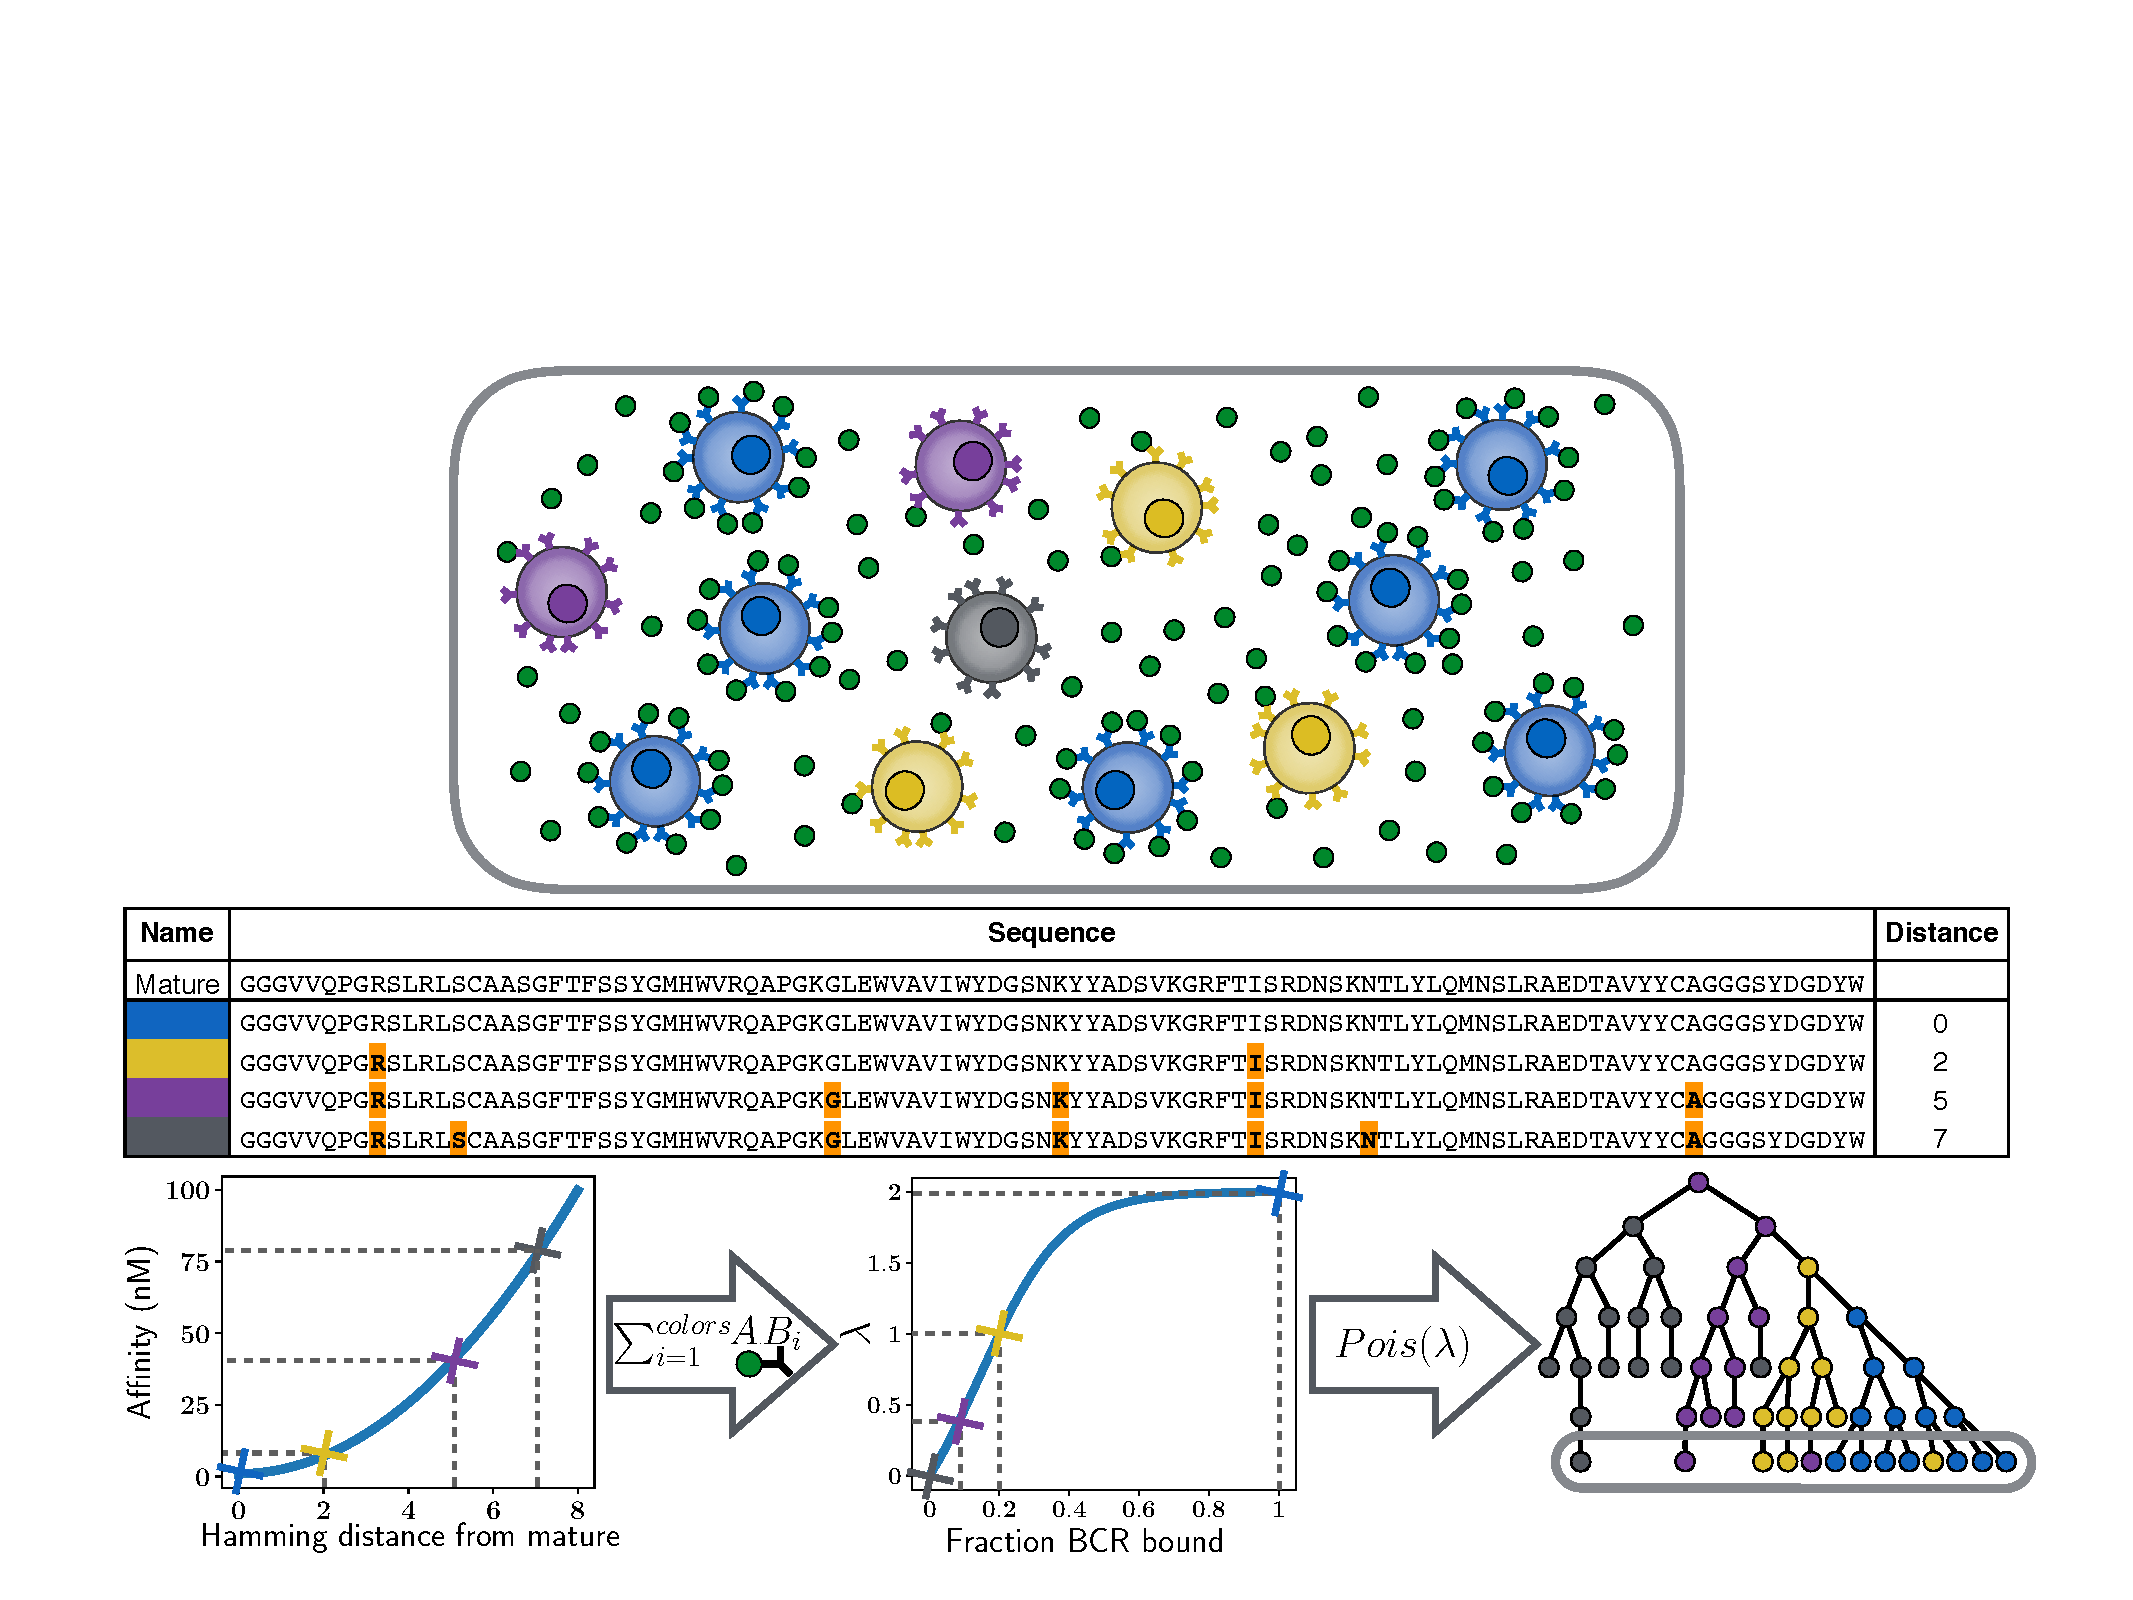
\includegraphics[width=1\textwidth]{figures/simulation_figure.pdf}
    \caption{
        \label{fig:simulation_figure}
        Simulation overview.
        The system is considered as a closed environment with free floating antigen and a number of B cells presenting BCRs on their surface, illustrated in the top panel.
        Different colors correspond to different affinity BCR sequences.
        In the middle panel a sequence alignment shows the distance between BCR sequences and the target mature BCR.
        Third panel shows first how distance from the mature BCR is used to find the affinity, next the fraction of bound BCRs is transformed to a $\lambda$ defining the progeny distribution.
        At the rightmost of panel three a tree is showing the lineage tree with an ellipse marking the B cells of the current generation also displayed in the first panel.
    }
\end{figure}






\subsubsection{Kinetic model of BCRs binding antigen}
Using the most simplistic view, B cells and antigens can be seen as molecules binding and unbinding at some rate intrinsic to the BCR sequences, and their dynamics can then be modelled as a continuously stirred tank reactor (CSTR) \cite{CSTR} widely used in chemical engineering.
The CSTR model makes the assumption that antigen is spread evenly across the GC and that the binding between BCRs and antigen is at equilibrium at all time.
In the following we derive the the fraction of B cell BCRs bound to antigen at steady state given these assumptions.


First let's consider what should constitute the measure of fitness in this system.
Fitness is related to amount of antigen bound and as an alternative to the total amount of bound antigen, we choose to normalize this number between 0 and 1 by using the fraction of BCRs bound to antigen.
Considering the BCRs as free molecules with a total concentration of $[B_{\total}]$, the fraction of BCRs bound to antigen at equilibrium is:
$$
B_{\bound} = \frac{[AB]}{[B_{\total}]}
$$
This B cell specific fitness measure will later be integrated into the simulation of the GC reaction, but for doing this we need to setup the CSTR system and derive its solution.


\noindent
We are modelling the binding equilibrium between free antigen ($[A]$), the free B cell receptor ($[B]$) and the two bound ($[AB]$):
\begin{equation}
\ce{[A] + [B] <=>[k_{\on}][k_{\off}] [AB]}
  \label{eq:bind1}
\end{equation}

\noindent
The on and off rate of binding is the expressed as constants $k_{\on}$ and $k_{\off}$. Affinity is the ratio of substrate and reactants at equilibrium, which is the same as the fraction between on vs.\ off rate:
\begin{equation}
K_d \equiv \frac{k_{\off}}{k_{\on}} = \frac{[A] [B]}{[AB]}
  \label{eq:Kd_def}
\end{equation}
%The law of mass conservation gives us that $B_{\total} = B + AB$.

\noindent
%Isolating $[AB]$ and substituting in the affinity definition $K_d$ from \eqref{eq:Kd_def}:
Isolating $[AB]$:
$$
[AB] = [B] \frac{[A]}{K_d}
$$

\noindent
Substituting $[B]$ for its expression from mass conservation, $[B_{\total}] = [B] + [AB]$:
$$
[AB] = ([B_{\total}] - [AB]) \frac{[A]}{K_d}
$$

\noindent
Which rearranges to:
$$
[AB] = \frac{[B_{\total}]}{1 + \frac{K_d}{[A]}}
$$

\noindent
Extending to multiple BCR affinities:
\[
 \begin{matrix}
  \ce{[A] + [B_1] <=>[k^1_{\on}][k^1_{\off}] [AB_1]} \\
  \ce{[A] + [B_2] <=>[k^2_{\on}][k^2_{\off}] [AB_2]} \\
  \vdots \\
  \ce{[A] + [B_n] <=>[k^n_{\on}][k^n_{\off}] [AB_n]}
  \label{eq:ABi}
 \end{matrix}
\]

\noindent
Affinity is a constant for each BCR and since all B cells compete for the same antigen, each $[AB_i]$ is dependent only through the concentration of unbound antigen:
\[
 \begin{matrix}
  [AB_1] = \frac{[B^1_{\total}]}{1 + \frac{K^1_d}{[A]}} \\
  [AB_2] = \frac{[B^2_{\total}]}{1 + \frac{K^2_d}{[A]}} \\
  \vdots \\
  [AB_n] = \frac{[B^n_{\total}]}{1 + \frac{K^n_d}{[A]}} \\
 \end{matrix}
\]

\noindent
Now introducing mass conservation for $A$:
\begin{equation}
A_{\total} = [A] + \sum_{i=1}^{n} [AB_i] \equiv [A] + \sum_{i=1}^{n} \frac{[B^i_{\total}]}{1 + \frac{K^i_d}{[A]}}
  \label{eq:A_objective}
\end{equation}
By rearranging to a polynomial form the system can be solved to find $[AB_i]$ for each B cell, afterwards transformed to $B^i_{\bound}$.
A solution will be elaborated in the implementation section.




\subsubsection{Transforming distance to target to affinity}
Next we describe how to simulate the affinity ($K_d$) of each BCR.
Potentially the affinities can be generated in any imaginable way by transforming a BCR sequence ($\Bseq$) into a number that represents affinity.
Formally this would be a function: $f(\Bseq_i) = K^i_d$.
In a realistic, yet still minimalistic, model we would imagine that the BCRs in a GC were evolving towards a specific target sequence denoted $\Tseq$.
A target is the sequence with the highest affinity, the state where fitness max out.
We will define a fitness landscape around the target using a distance function, $\operatorname{dist}(\cdot,\cdot)$, which we assume to be given as the Hamming distance between amino acid sequences.

Let's define the affinity of the naive input sequence as $K^{\naive}_d$ and correspondingly the affinity for the mature target sequence as $K^{\mature}_d$.
Now we can define an arbitrary function with reference points in $K^{\naive}_d$ and $K^{\mature}_d$, that transforms a distance between $\Bseq$ and $\Tseq$ to an affinity:
$$
\Affinity(\Bseq, \Tseq, K^{\naive}_d, K^{\mature}_d) = K^i_d
$$
There are two conditions we want to impose.
If the BCR sequences is equal to the naive sequence ($\Nseq$), then it takes the affinity of the naive BCR, and if it is equal to the mature target sequence ($\Tseq$), it takes the affinity of the mature BCR:
\begin{equation}
\begin{split}
\Affinity(\Nseq, \Tseq, K^{\naive}_d, K^{\mature}_d) = K^{\naive}_d \\
\Affinity(\Tseq, \Tseq, K^{\naive}_d, K^{\mature}_d) = K^{\mature}_d
\end{split}
\label{eq:hd2affy_cond}
\end{equation}
These conditions are satisfied by:
\begin{equation}
\Affinity(\Bseq, \Tseq, K^{\naive}_d, K^{\mature}_d) = K^{\mature}_d + \left ( \frac{d}{t_{\naive}} \right )^k (K^{\naive}_d - K^{\mature}_d)
\label{eq:hd2affy}
\end{equation}
Where $d = \operatorname{dist}(\Bseq, \Tseq)$ is the distance between input and target sequence and $t_{\naive} = \operatorname{dist}(\Nseq, \Tseq)$ is the distance between naive and target sequence.
The exponent, $k$, can be chosen to adjust the mapping between distance and affinity, with the restriction that $0 < k < \infty$ (figure \ref{fig:hd2affy}).

\begin{figure}[!h]
    \centering
    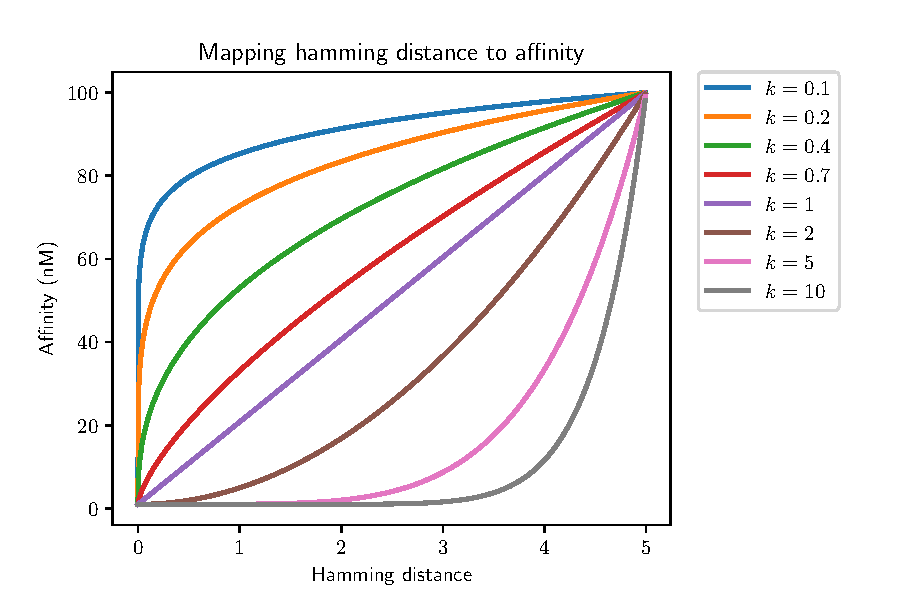
\includegraphics[width=0.9\textwidth]{figures/hd2affy.pdf}
    \caption{
        \label{fig:hd2affy}
        Varying the exponent $k$ in \eqref{eq:hd2affy} to achieve different mappings between distance and affinity.
        Naive and mature affinity is held constant, $K^{\naive}_d = 100nM$ and $K^{\mature}_d = 1nM$.
    }
\end{figure}


It is easy to imagine that in a real affinity maturation process there will be many different BCR sequences that are practically equally fit.
E.g.\ this will happen when multiple amino acids are equally fit on a given position, and it will also happen if there are multiple distinct maturation paths that ends up with equally fit BCRs.
The later effect can be introduced into the model be adding multiple target sequences and then determining the affinity based on the shortest distance to any of these:
$$
d = \argmin_{\Tseq \in \Targets} \operatorname{dist}(\Bseq, \Tseq)
$$




\subsubsection{Transforming BCR occupancy to fitness}
In the affinity model the fitness of a B cell is determined by the amount of antigen it has bound divided by the total number of receptors it has ($B^i_{\bound}$).
%In the affinity model the fitness of a B cell is determined by the amount of antigen it has bound divided by the total number of receptors it has, we shall call this $B^i_{\bound}$ for the BCR $B_i$.
The progeny distribution should adjust according to $B^i_{\bound}$, so if $B^i_{\bound}$ is small the progeny distribution should favor terminating the B cell and opposite, if $B^i_{\bound}$ is large this should cause the progeny distribution to favor cell division.
The Poisson distribution will reflect this behaviour by setting $\lambda_i$ small when $B^i_{\bound}$ is small and $\lambda_i$ large when $B^i_{\bound}$ is large.
To use $\operatorname{Pois}(\lambda_i)$ as the progeny distribution we need a function transforming $B^i_{\bound}$ to $\lambda_i$: $Y(B^i_{\bound}) = \lambda_i$.
For this purpose we can use a generalized version of the logistic function since it has the properties we need:
\begin{equation}
\lambda_i = Y(B^i_{\bound}) = \alpha + \frac{K - \alpha}{G + Q \exp(-\beta B^i_{\bound})}
  \label{eq:BA_trans}
\end{equation}
$G$ is chosen to be the typical value of $1$.
$K$ is the upper bound of the function and is set to $2$, reflecting that the fastest average growth is $2^t$, with $t$ generations (setting $\operatorname{max}(\lambda) = 2$ is a model choice, but could be changed).
$\alpha$, $\beta$ and $Q$ are fit to fulfill three conditions:
\begin{equation}
Y(0) = 0, \ \ \ Y \left(\frac{f_{\full}}{U} \right) = 1, \ \ \ Y(f_{\full}) = 2 - \epsilon
  \label{eq:BA_cond}
\end{equation}
The solution is undefined in $Y(f_{\full}) = 2$ because the function is asymptotically growing towards 2, therefore $\epsilon$ can be regarded as a small value (e.g.\ $10^{-3}$) so that $Y(f_{\full}) \approx 2$.
$0 < f_{\full} \leq 1$ is the fraction of bound BCRs ($B^i_{\bound}$) sufficient to make the B cell fully activated.
At $f_{\full}$ the highest fitness is achieved and binding more antigen will not change the progeny distribution, ignoring the negligible contribution of $\epsilon$.
The constant $U > 1$ in condition 2 can be adjusted to set the value of $B^i_{\bound}$ resulting in $\lambda_i = 1$.
The interpretation of $U$ is that it is the fraction of BCRs binding antigen necessary to sustain the life of the B cell.
Using these conditions $\alpha$, $\beta$ and $Q$ can be found and the logistic function is fully defined.
% $\alpha$ can be interpreted as the lower asymptote of the function and is therefore expected to be close to 0, except the case when $U$ is large, in which $\alpha$ has to adjust to a larger negative value, see figure \ref{fig:T_Bbound_U}.
$\alpha$ can be interpreted as the lower asymptote of the function.
$\beta$ is the steepness of the function and it is coupled to the $Q$ parameter and follow it according to the three conditions in \eqref{eq:BA_cond}.

\begin{figure}[!ht]
    \centering
    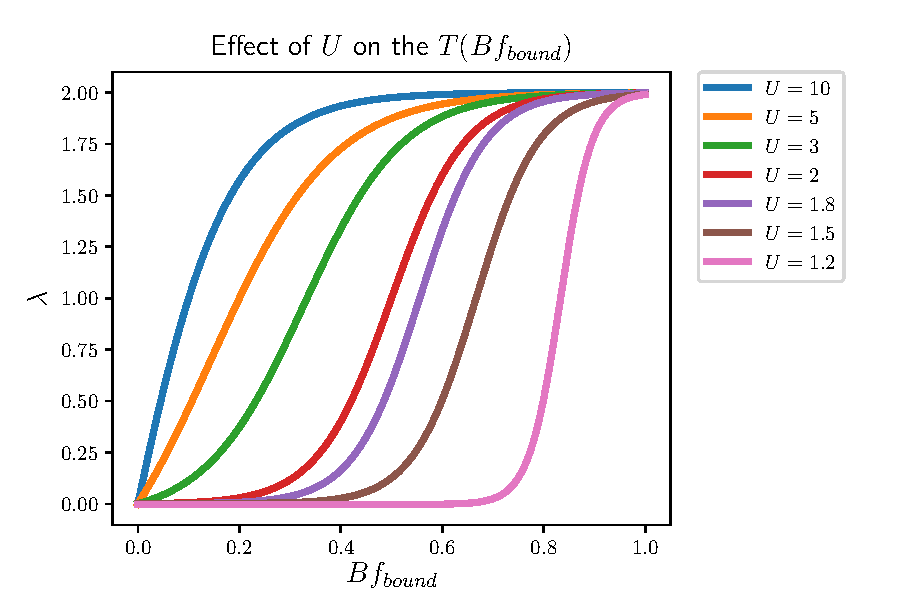
\includegraphics[width=0.8\textwidth]{figures/T_Bbound_U.pdf}
    \caption{
        \label{fig:T_Bbound_U}
        Using a constant $f_{\full} = 1$, changing the $U$ parameter in the conditions in \eqref{eq:BA_cond} to achieve a shift of the inflection point at $\lambda=1$ on the $B_{\bound}$ axis.
    }
\end{figure}

\begin{figure}[!ht]
    \centering
    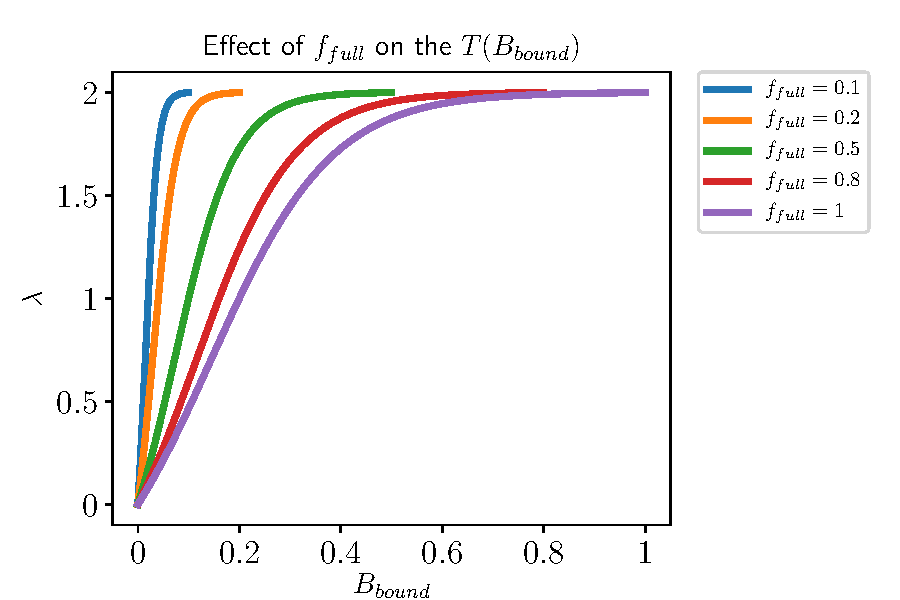
\includegraphics[width=0.8\textwidth]{figures/T_Bbound_f_full.pdf}
    \caption{
        \label{fig:T_Bbound_f_full}
        Using a constant $U = 5$, changing the $f_{\full}$ parameter in the conditions in \eqref{eq:BA_cond} to change the point where $B_{\bound}$ reaches the $\lambda$ plateau.
    }
\end{figure}


\iffalse
\begin{figure}
    \centering
    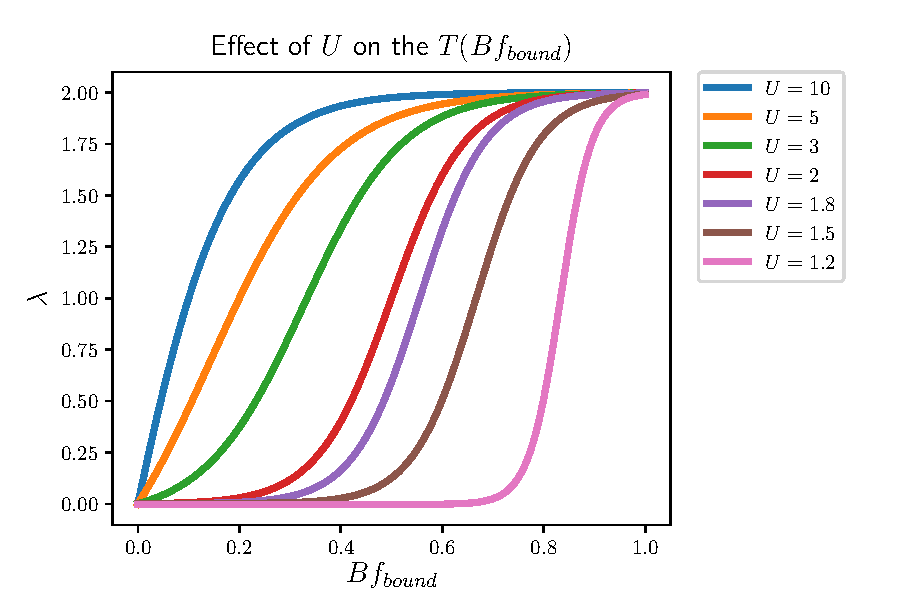
\includegraphics[width=0.8\textwidth]{figures/T_Bbound_U.pdf}
    \caption{
        \label{fig:T_Bbound_U}
        Using a constant $f_{\full} = 1$, changing the $U$ parameter in the conditions in \eqref{eq:BA_cond} to achieve a shift of the inflection point at $\lambda=1$ on the $B_{\bound}$ axis.
    }
    \centering
    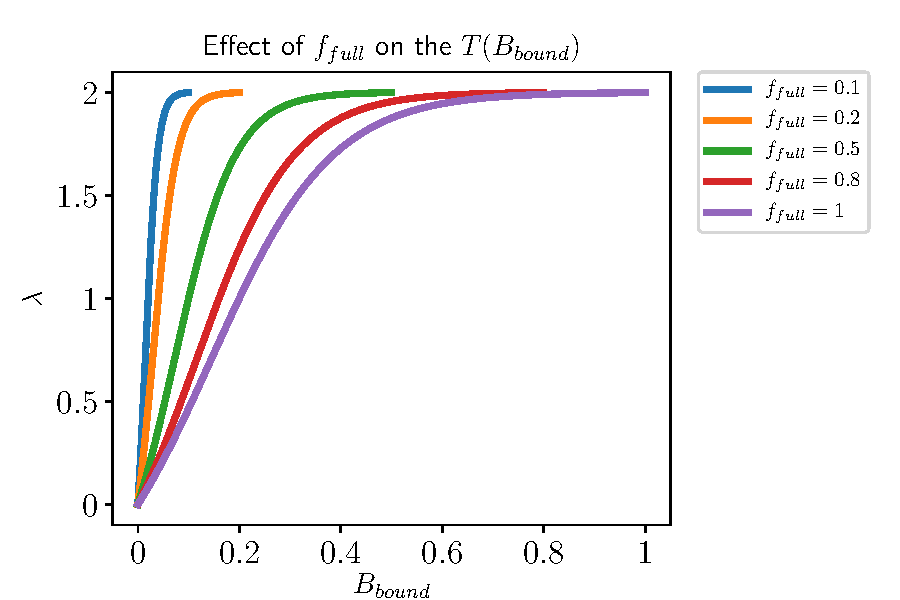
\includegraphics[width=0.8\textwidth]{figures/T_Bbound_f_full.pdf}
    \caption{
        \label{fig:T_Bbound_f_full}
        Using a constant $U = 5$, changing the $f_{\full}$ parameter in the conditions in \eqref{eq:BA_cond} to change the point where $B_{\bound}$ reaches the $\lambda$ plateau.
    }
\end{figure}
\fi




\subsubsection{The carrying capacity of a GC}
Finally we need to introduce the concept of a carrying capacity of a GC, which is defined as the number cells a GC is able to support in its micro environment.
The carrying capacity is determined mainly by the total concentration of antigen since binding to antigen controls the progeny distribution.
BCR affinity is also influencing antigen binding and therefore must influence the carrying capacity, but at high affinity nearly all antigens are bound and hence the total antigen concentration is the most influential determinant of GC carrying capacity.
At $\operatorname{Pois}(1)$ the progeny distribution is only just sustaining the population size of the GC, and given condition 2 in \eqref{eq:BA_cond} this happens at $\frac{f_{\full}}{U}$.
Under the assumption that the population of B cells all have identical BCR sequences, the maximum carrying capacity is:
\begin{equation}
C([A_{\total}]) = U \frac{[A_{\total}] - [A]}{f_{\full}}
  \label{eq:carry_cap}
\end{equation}
The concentration of unbound antigen is determined by the affinity and concentration of BCRs.
It is fair to assume that there are many more BCRs than antigens, so for high affinity BCRs the majority of antigen should be in a bound state allowing for the approximation of setting $[A]=0$.
This makes it easy to calculate the carrying capacity given \eqref{eq:carry_cap}.
However in the cases with low affinity the concentration of free antigen cannot be assumed zero and in such cases $[A]$ should be determined through \eqref{eq:A_objective}.

In the situation where a newly arising mutant has higher affinity than the rest of the population the fraction of BCRs binding antigen on this mutant will approach $f_{\full}$, resulting in a high probability that the clone will expand rapidly to overtake the GC population, also known as a clonal burst.
The clonal burst has the characteristic time (average time of take over) being:
$$
T_{\burst} = \log_2 \left(\text{carrying capacity} \right) = \log_2\left( U \frac{[A_{\total}] - [A]}{f_{\full}} \right)
$$
% With $\kappa = \operatorname{max}(\lambda) = K$ but in this model fixed to $K=2$ and $U$ and $f_{\full}$ being constants defined in the next section.






\subsection{Parameter choice}
We chose the parameter $U$ in the logistic transformation to take a value that reflects our belief of how the shape of this transformation should look.
Our expectation is that initially, when only a few BCRs are bound and stimulation is low, there will be a linear increase of the stimulus with increasing antigen binding.
At some point close to $f_{\full}$, this increase in stimulus should level out because the cell can only be stimulated to $\operatorname{max}(\lambda)=2$.
This expected shape is recapitulated by a choosing $U=5$, see figure \ref{fig:T_Bbound_U}, and therefore this is where we fix $U$.

The choice of $f_{\full}$ determines the BCR occupancy when full activation of proliferation is achieved.
$f_{\full}$ does not have any known reference value so it is chosen to take a value of 1 because this is mathematically convenient.
It turns out that the model is quite robust to different choices of $f_{\full}$ and it causes no substantial effect to change it from 1 to 0.05 (figure \ref{fig:no_effect_of_f_full}) justifying our choice.
Changing $f_{\full}$ will primarily effect the carrying capacity via \eqref{eq:carry_cap}, but by adjusting $[A_{\total}]$ to get the same carrying capacity simulations are indifferent to the choice of $f_{\full}$.
Presumably this is because the shape of the logistic transformation $Y(\cdot)$ in \eqref{eq:BA_trans} will remain intact (figure \ref{fig:T_Bbound_f_full}).
The choice of $f_{\full} = 1$ has the interpretation that when $\frac{1}{U}$ of the BCRs on a B cell are binding antigen it has a $\operatorname{Pois}(1)$ progeny distribution, and when all BCRs are binding antigen the progeny distribution increases to $\operatorname{Pois}(2-\epsilon)$.

\begin{figure}[!ht]
\begin{center}
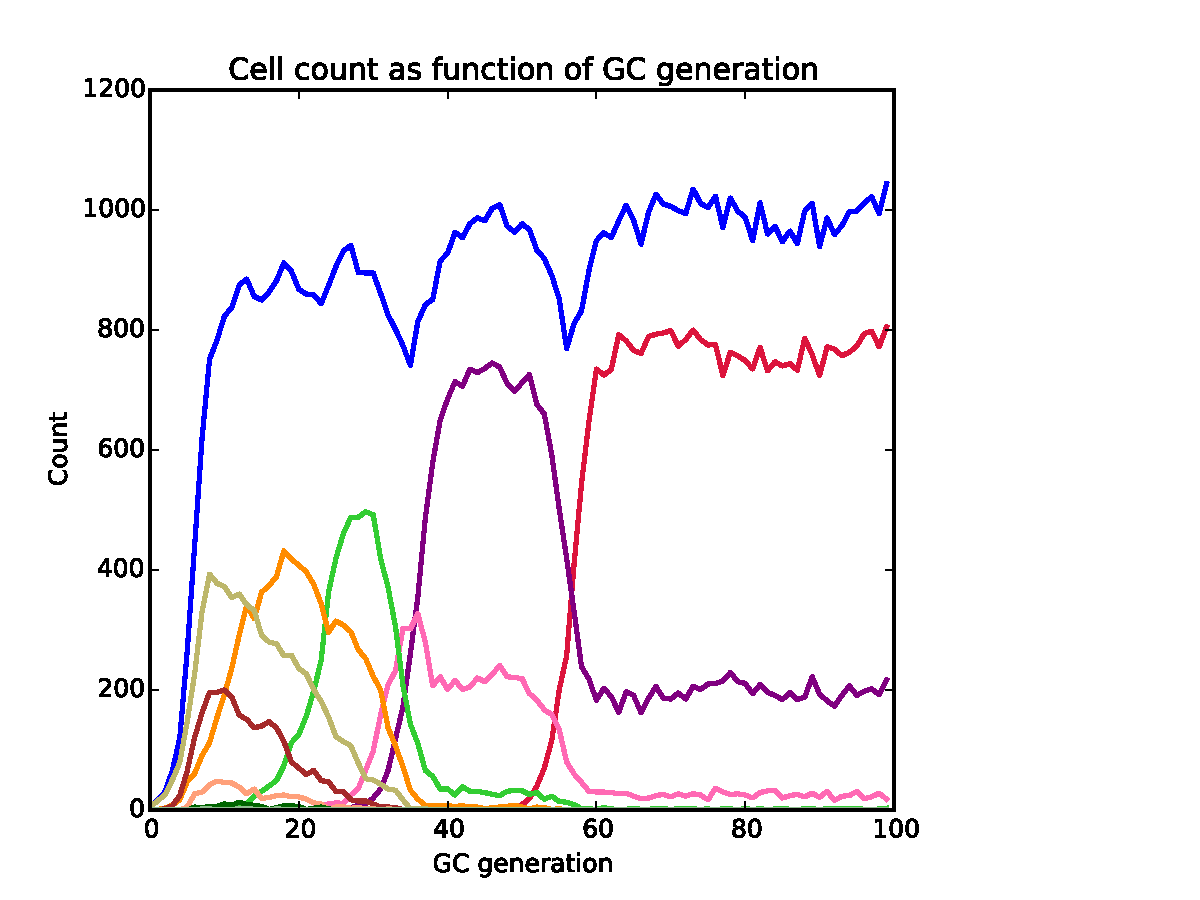
\includegraphics[height=49mm]{figures/f_full_1.pdf}
%\hspace{-40mm}
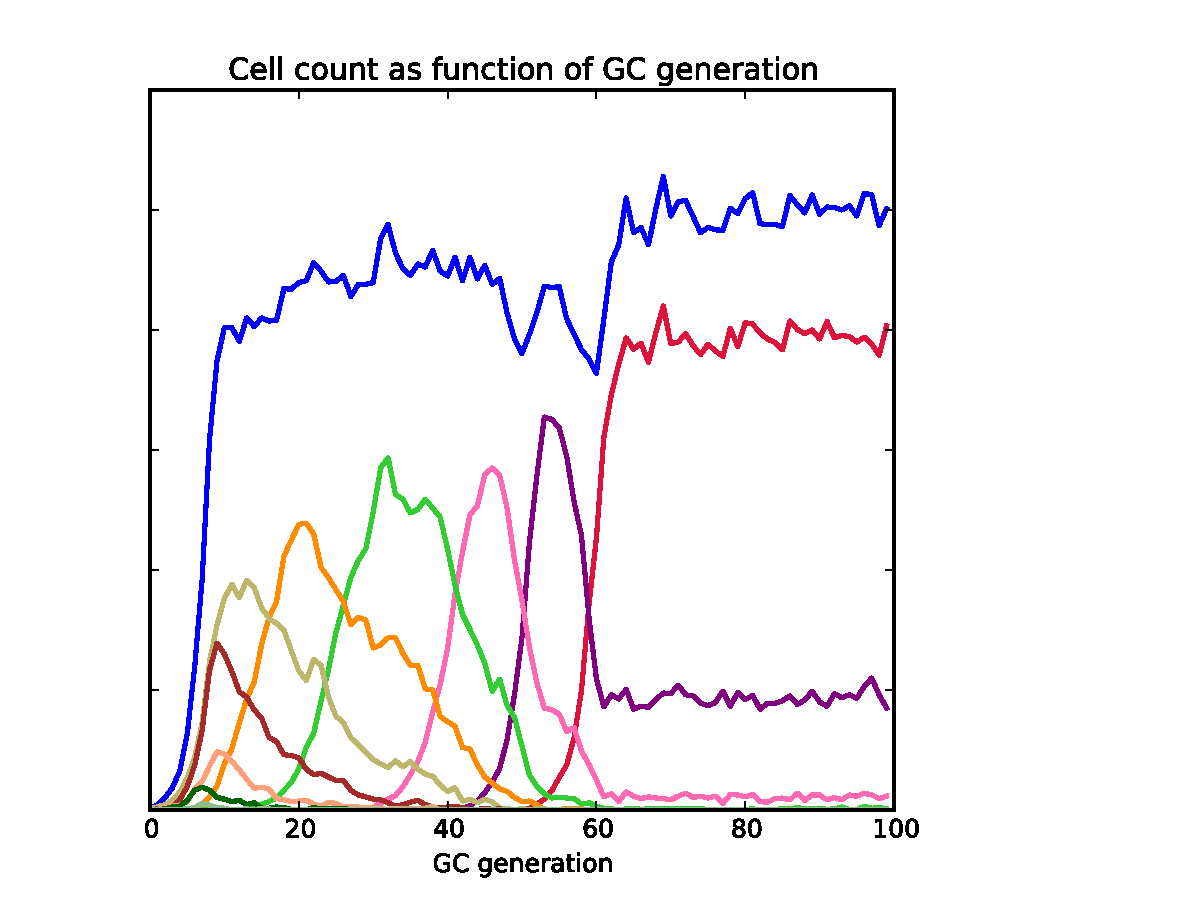
\includegraphics[height=49mm]{figures/f_full_05.pdf}
%\hspace{-40mm}
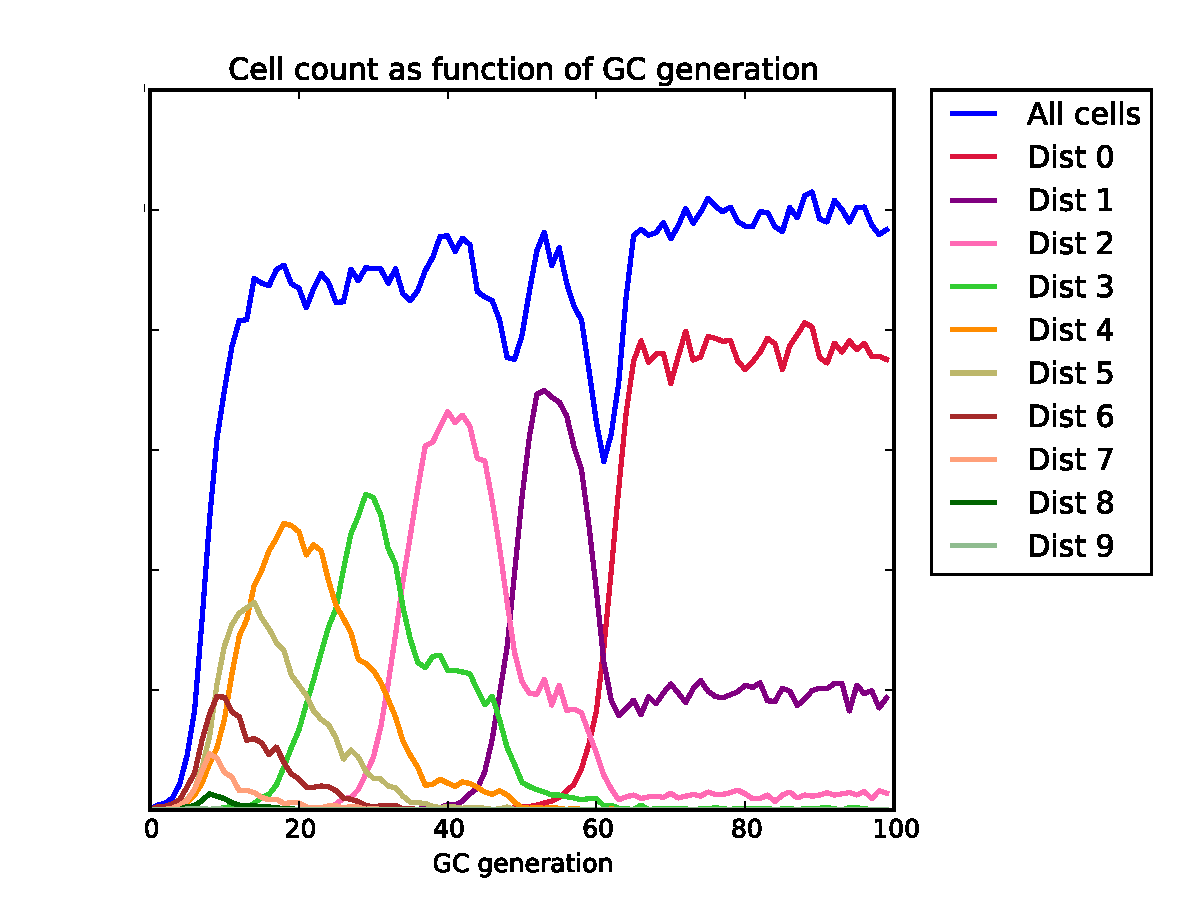
\includegraphics[height=49mm]{figures/f_full_005.pdf} \newline%
\end{center}
\vspace{-8mm} \hspace{23mm} (a) \hspace{37mm} (b) \hspace{37mm} (c)
    \caption{
        \label{fig:no_effect_of_f_full}
        Simulation with affinity selection for varying magnitudes of $f_{\full}$.
        $f_{\full}=1$, $f_{\full}=0.5$, $f_{\full}=0.05$ for (a), (b) and (c) respectively.
        Simulations with $U=5$ and $[A_{\total}]$ adjusted to obtain a carrying capacity of 1000 cells.
        Each simulation is run for 100 generations with $t_{\naive}=10$ and the composition of sequence distances to their closest targets are plotted for each generation.
        }
\end{figure}


In the transformation from distance to affinity in \eqref{eq:hd2affy}, we have to make a choice about which exponent to use.
There is reason to believe that not all mutations are improving affinity with equal proportion and therefore the linear transformation is excluded.
Another thing we would like to enforce is to disallow sequences to drift far away from both the mature and naive sequence.
A large sequence drift should not be very likely since it would completely abolish the binding of antigen and therefore it is preferred to have an exponent $k>1$.
We choose $k=2$ since this puts an extra penalty on simulated sequences that are drifting, without putting an excessive emphasis on the first two steps of approaching the mature sequence, see \ref{fig:hd2affy}.

The logistic function is chosen to yield a maximum $\lambda$ of 2 since this would correspond to an average max progeny of 2 cells per generation, yielding a standard exponential population growth of $2^t$.
One useful feature of the logistic function is that it has a notion of maximum signal i.e.\ when more antigen binding does not give more signal.
It is asymptotically approaching 2 which means that the maximum growth rate of $\lambda=2$ is not reached completely at $f_{\full}$.
To fit the function we have to allow for this by choosing a small $\epsilon$ that makes $Y(f_{\full})$ practically equivalent to 2.
Here we choose $\epsilon=\frac{1}{1000}$ meaning that $Y(f_{\full}) = \frac{1999}{1000}$.

Next we need to find some realistic numbers for the constants such as affinity, carrying capacity and $B^i_{\total}$.
First let's consider affinity.
$K_d$ for a naive sequence is likely in the low micro molar range range of $10^{-6} - 10^{-7} M$, while the mature affinity is in the nano or subnano molar range of $10^{-8} - 10^{-10} M$ \cite{berek1987mutation} ($M$ is used to denote molar concentration).
Classically these affinity measurements have been done using hapten induced immunizations, and there is reason to believe that conclusions about affinities will be different for other antigens.
Indeed it has been reported that naive sequences in some cases can be high affinity binders making affinity maturation less useful \cite{frank2015simple}.
Nevertheless, several groups have reported 50-100 fold affinity increase due to affinity maturation in both complex and hapten induced immunizations \cite{Kelsoe_2016}, \cite{phan2006high}, \cite{ulrich1997interplay}.
We choose the naive sequence to be $10^{-7} M$ ($100nM$) and the mature to be $10^{-9} M$ ($1nM$), giving a large span in affinity to select on.

With the introduction of $K_d$'s we need to consider units.
Let's start by estimating the concentration of BCRs per B cell in the GC, also denoted as $B^i_{\total}$.
To simplify things we assume that the number of BCRs on each B cell is the same.
In each GC there is an estimated $4 \times 10^3$ B cells \cite{kroese1990germinal}, but it has before been estimated to just $1000$ \cite{Childs_Baskerville_Cobey_2015} which we will use for convenience.
On the surface each of these B cells have an estimated $10^4$ BCRs \cite{rieckmann2017social}, \cite{immprot} (highly uncertain estimate), resulting in $10^7$ BCRs per GC.
Converting this to moles gives: $10^7\ 6 \times 10^{-23} \text{moles}$
The GC is reported to have a diameter of $10^{-4} m$ \cite{Romppanen_1981}.
Assuming the shape is spherical and converting to liters gives:
$$
\frac{4}{3} \pi \left(\frac{1}{2} \times 10^{-4} m \right)^3 10^3 \frac{L}{m^3} = \frac{1}{6} \pi \times 10^{-9} L
$$
Finally this gives:
$$\frac{10^7\ 6 \times 10^{-23} \text{moles}}{\frac{1}{6} \pi 10^{-9} L} \approx 10^{-6} M \equiv 10^{3} nM
$$
This means that each B cell contributes approximately $1nM$ to the total concentration of BCRs.
Now to simplify things everything is normalized to nano molar so e.g.\ the naive/mature affinity is changed to $100nM$ and $1nM$ respectively.
All the above described values are tabulated in table \ref{constants} and used as constants in later simulations of sequences undergoing affinity selection.

%We then make the assumption that the total concentration of antigen is equal to half of the total amount of BCRs in a fully grown GC with $10^3$ B cells each having $10^4$ BCRs.
%This makes a convenient reference point which is not unrealistic and we shall see later that the outcome of the simulations are rather insensitive to the concentration of antigens over a certain threshold.
%By looking at the definition of $[AB_n]$ it can be seen that changing the total concentration of antigen has the same effect as shifting the affinity of both the naive and mature sequence by the same fraction and this is the way it can easily be investigated.
%   - With the side effect of increasing the carrying capacity.


\begin{table}[ht]
\centering
\begin{tabular}{llll}
Constant    & Value & Description & Reference \\ \hline
$B^i_{\total}$ & $1\times10^{4}$     & Number of BCRs on each B cell & \cite{immprot}, \cite{rieckmann2017social}*     \\
$n_t$ & 1000 & B cells per GC &  \cite{kroese1990germinal}, \cite{Childs_Baskerville_Cobey_2015} \\
d & $10^{-4} m$ & GC diameter &  \cite{Romppanen_1981} \\
$\frac{1}{U}$           & $\frac{1}{5}$     & Fraction of $f_{\full}$ necessary to sustain the population & See text \\
k           & 2     & Exponent of affinity transformation & See text  \\
$f_{\full}$  & 1     & Fraction BCRs bound at full response & See text \\
$K_d^{\naive}$ & 100nM & Naive affinity & \cite{berek1987mutation} \\
$K_d^{\mature}$ & 1nM & Mature affinity & \cite{berek1987mutation} \\
\end{tabular}
\caption{
\label{constants}
    Constants used in the model of affinity selection. *There is a lot of uncertainty in this number and depending on the method it is estimated from $10^3$ to $10^7$.}
\end{table}









\subsection{Implementation}
In the solution to the BCR antigen binding equilibrium in \eqref{eq:A_objective} B cells with the same BCR sequence are included in the same $B^i_{\total}$, and hence the $B^i_{\total}$ will be different when some B cell genotypes are highly abundant while others are less.
To simplify bookkeeping let's expand the index, $i$, to represent just a single B cell, resulting in the simplification that $[B^1_{\total}] = [B^2_{\total}] = \ldots = [B^i_{\total}]$.
%The index, $i$, has then changed from a BCR genotype index to a B cell index.
In this notation multiple B cells can have the same BCR sequence, but each will have their own index because they are associated with different B cells.
This simplifies bookkeeping because the BCR index is always the same as the B cell index.
The change does not affect the solution in \eqref{eq:A_objective}.
Now given some total concentration of antigen, $A_{\total}$, the solution to the concentration of free antigen at equilibrium, $[A]$, reduces to finding the real positive root of the polynomial in \eqref{eq:A_objective}.
Finding this root is easily be done using Newton's method or by using a faster method like the Broyden–Fletcher–Goldfarb–Shanno (BFGS) algorithm \cite{shanno1985broyden}.
Once $[A]$ is found we can obtain the concentration of bound antigen by plugging it into \eqref{eq:ABi}.
Lastly $B_{\bound}$ is converted to a progeny distribution parameter $\lambda$ by using \eqref{eq:BA_trans}.

All the above model definitions have the single purpose of adjusting the progeny distribution of a cell through $\lambda_i$, given some fitness function.
Under the neutral model this fitness function is constant, resulting in the same $\lambda_i$ for all cells, while in the affinity selection model $\lambda_i$'s are updated to reflect B cell fitness in a GC reaction.
Practically the simulation of sequences can be thought of as a process of constructing a phylogenetic tree, see figure \ref{fig:tree_iteration}.
In each generation an integer is drawn from each of the progeny distributions for all non terminated leaves on the tree.
The leaf can then either terminate or have $1$ to $N \in \Z_+$ progeny cells.
If the leaf has progeny each will undergo their own mutation process following the S5F model and become leaves in the next generation.
One generation is defined as one iteration through all the non terminated leaves on the tree and this is done in random order to avoid any bias.
Once every leaf has been evaluated this marks a new generation and the generation time is increased by one.
For an overview see figure \ref{fig:tree_iteration}.

\begin{figure}[!ht]
    \centering
    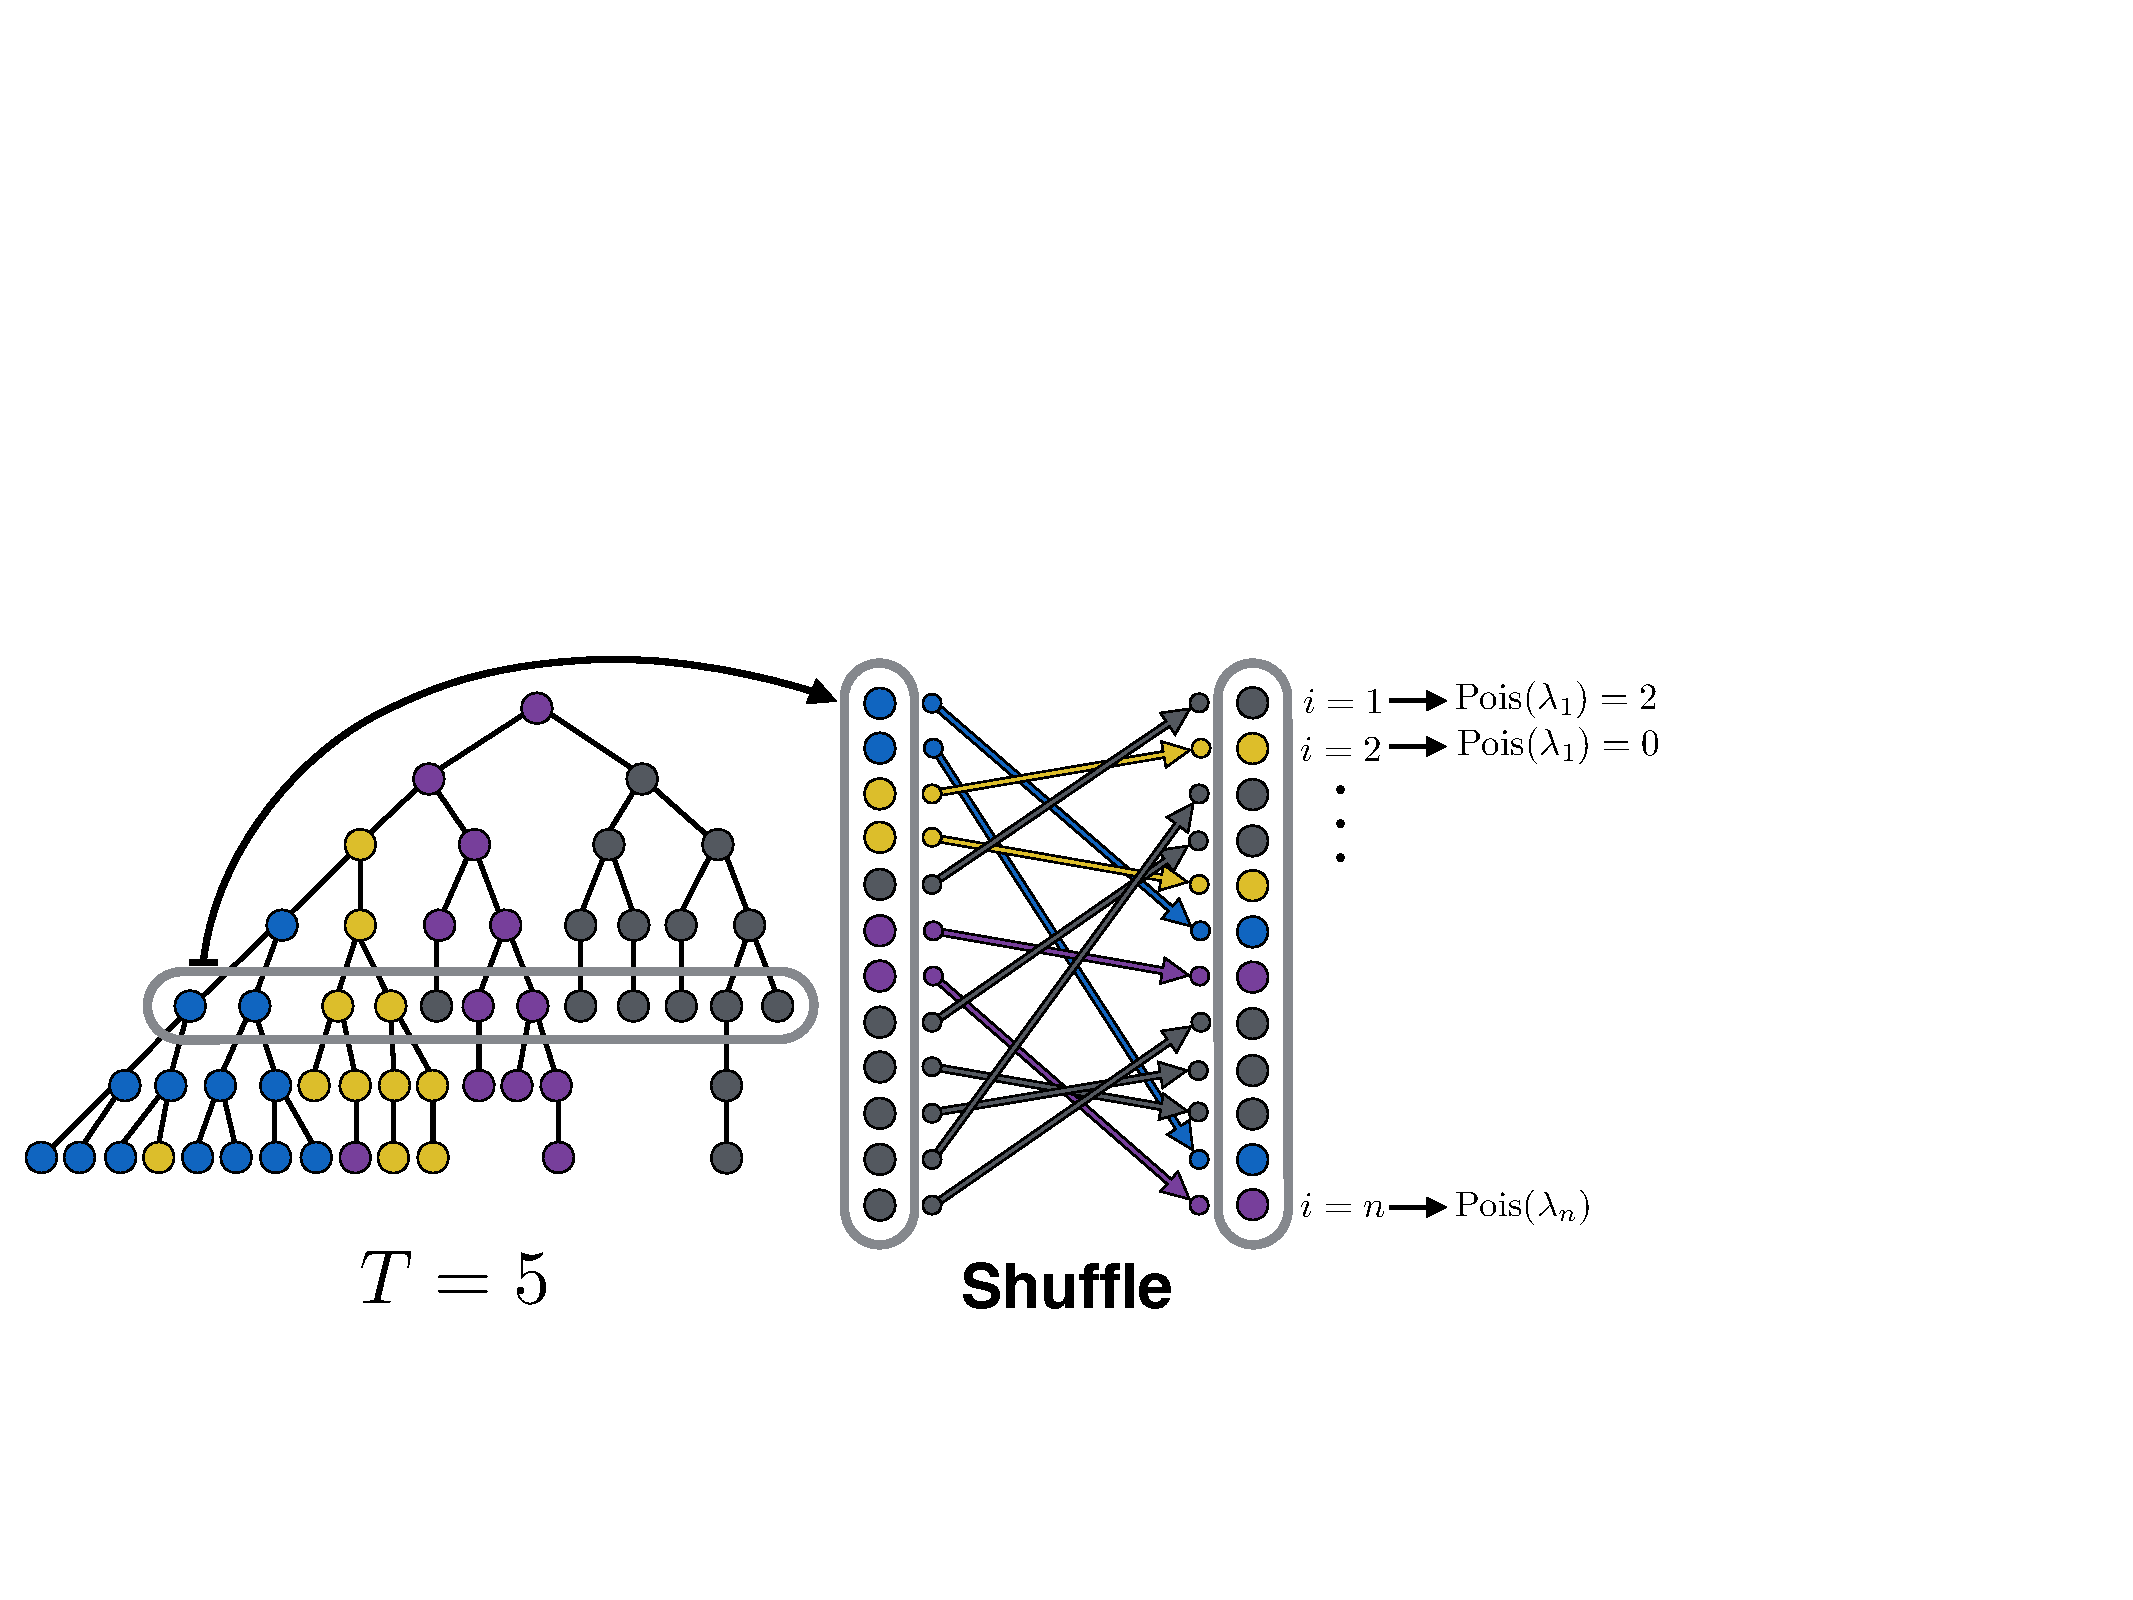
\includegraphics[width=0.9\textwidth]{figures/tree_iteration.pdf}
    \caption{
        \label{fig:tree_iteration}
        Illustration the sampling procedure in a time slice ($T=5$) of the simulation of a phylogeny undergoing affinity selection.
        A generation time is defined as the time when all nodes have been sampled and their progeny has been evaluated.
        At each generation all non-terminated nodes will be evaluated in random order.
        For neutral selection $\lambda_i$ is constant and identical for all cells.
        For simulation with affinity selection $\lambda_i$ is B cell dependent and re-evaluated every time there is a change in the population of non-terminated nodes.
        % This re-evaluation of all the $\lambda$s that can be skipped for a number of nodes to save computation time without any substantial difference in simulation characteristics.
    }
\end{figure}


Using tree terminology, the progeny distribution of a leaf depends on all the states (i.e.\ sequences) of the non terminated leaves.
Then by definition the affinity model needs to be updated, by re-evaluating \eqref{eq:A_objective} and finding all $[AB]_i$, every single time a new leaf is generated, creating a computational burden for large population sizes.
In simulations with a carrying capacity of 1000 cells, the vast majority of the computations are spent updating $[AB]_i$.
An approximate solution is simply to skip some of these updates and rely on the previous determination of $\lambda_i$, as an example a system with 1000 cells could be update only at every 100th cell progeny evaluation, resulting in only 10 evaluations per generation and orders of magnitude faster runtime.
Regardless of whether evaluations are skipped, all $\lambda_i$'s will be updated when a new generation is started.
The rationale behind skipping evaluations is that when there is already a large population of cells, then very little will change after a single cell is added.
In fact it turns out that for simulations using a carrying capacity of 1000 cells, there are no distinct difference between updating $[AB]_i$ after every leaf is evaluated or once every 100th leaf progeny evaluation (figure \ref{fig:skip_vs_no_skip_dist10}).

\begin{figure}[!ht]
\begin{center}
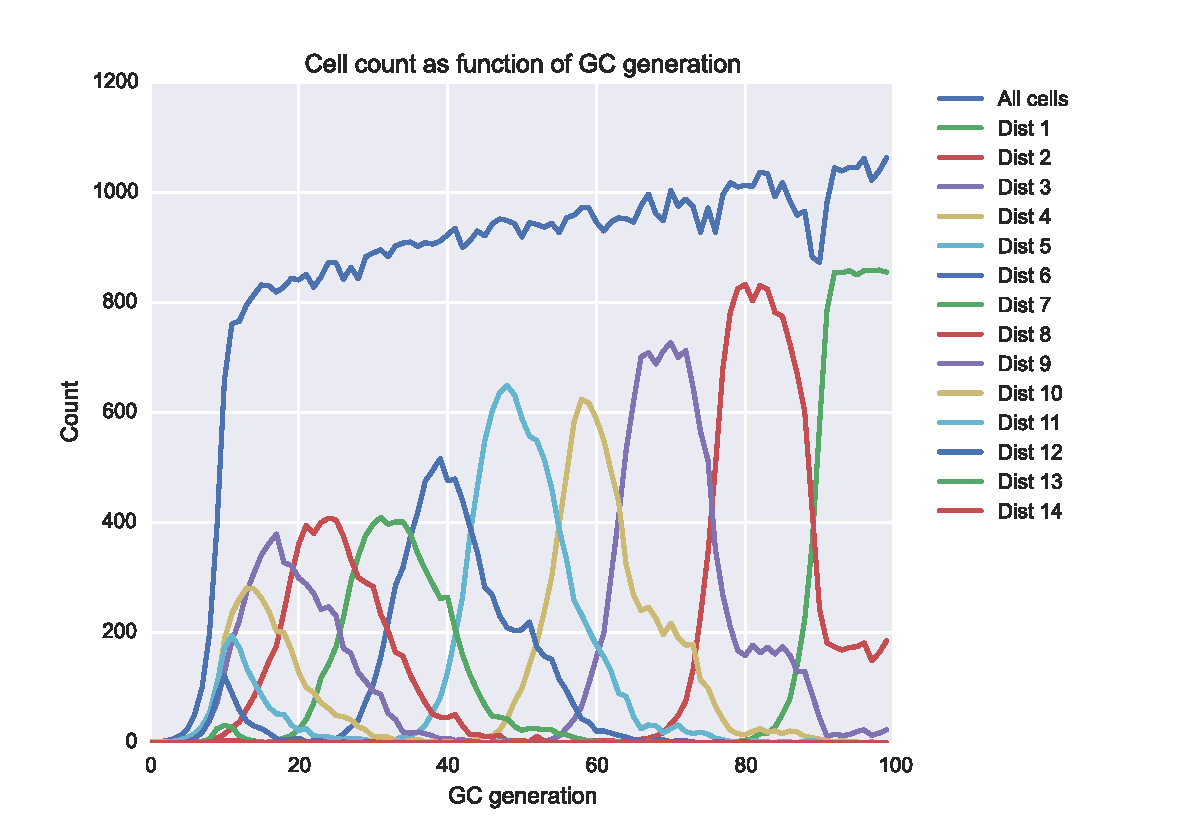
\includegraphics[width=80mm]{figures/sim_selection_default_run_dist10.pdf}
\hspace{-22mm}
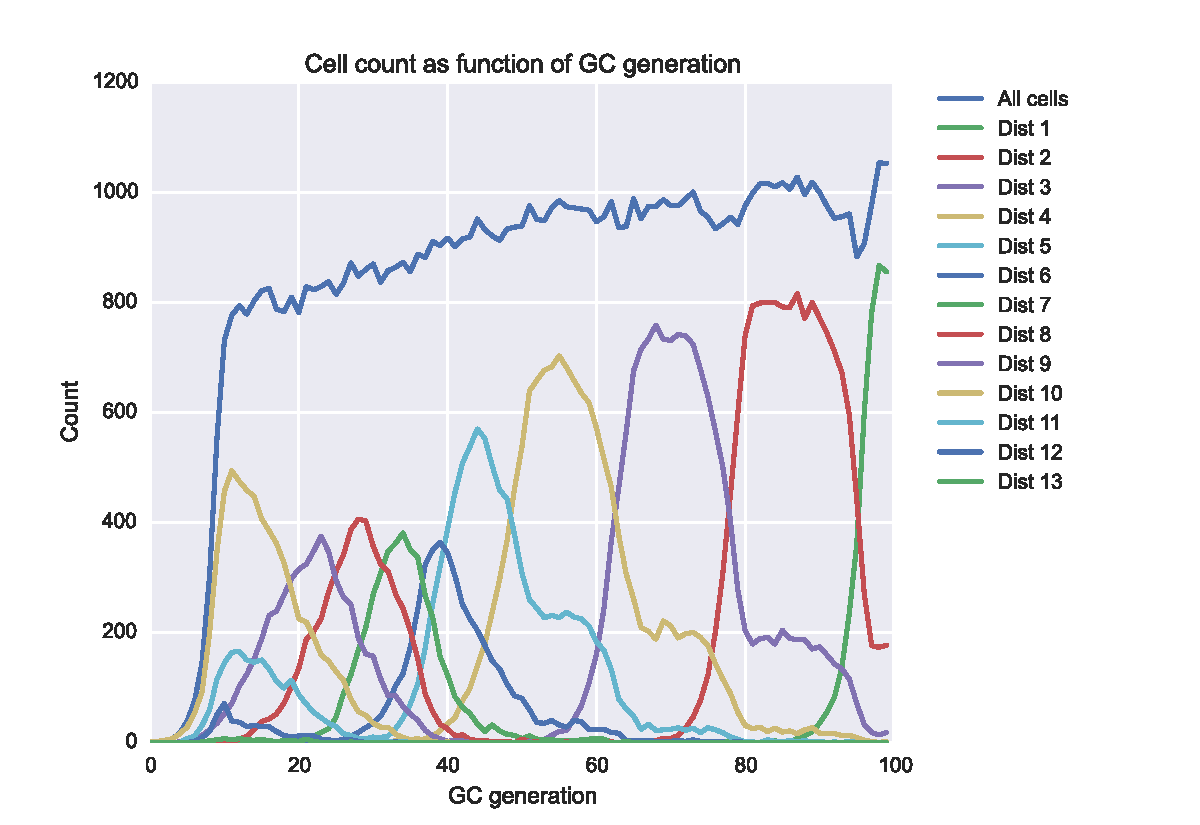
\includegraphics[width=80mm]{figures/sim_selection_default_run_dist10_no_skip.pdf} \newline%
\end{center}
\vspace{-9mm} \hspace{34mm} (a) \hspace{53mm} (b)
    \caption{
        \label{fig:skip_vs_no_skip_dist10}
        Simulation with selection comparing (a) with and (b) without skipping recalculations of $\lambda_i$ at each cell evaluation.
        In (a) no steps are skipped while, in (b), 99\% of all recalculations are skipped (10 updates to a population of 1000 B cells).
        Simulation parameters are default as in table \ref{aff_constants} with $\lambda_{\mut} = 0.3$ and $T=100$.
        }
\end{figure}

\iffalse
\begin{figure}[!ht]
\begin{center}
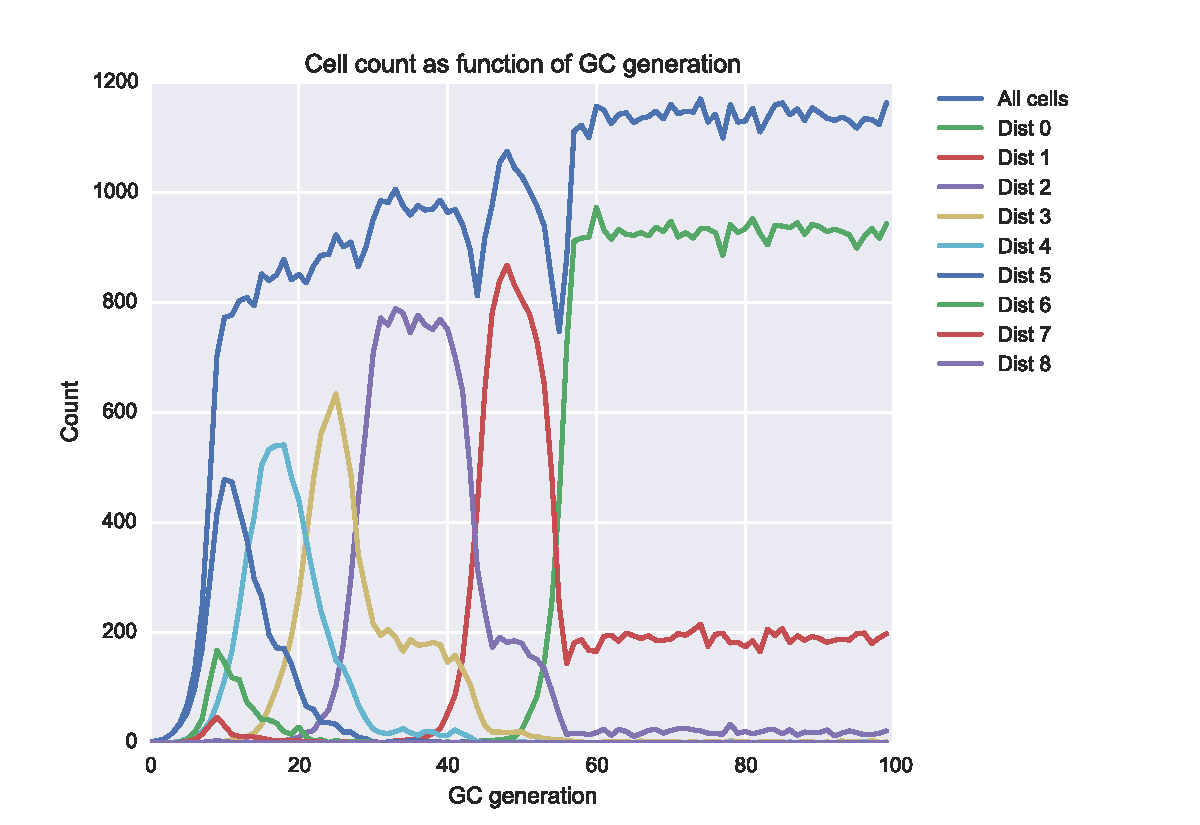
\includegraphics[width=80mm]{figures/sim_selection_default_run_dist5.pdf}
\hspace{-20mm}
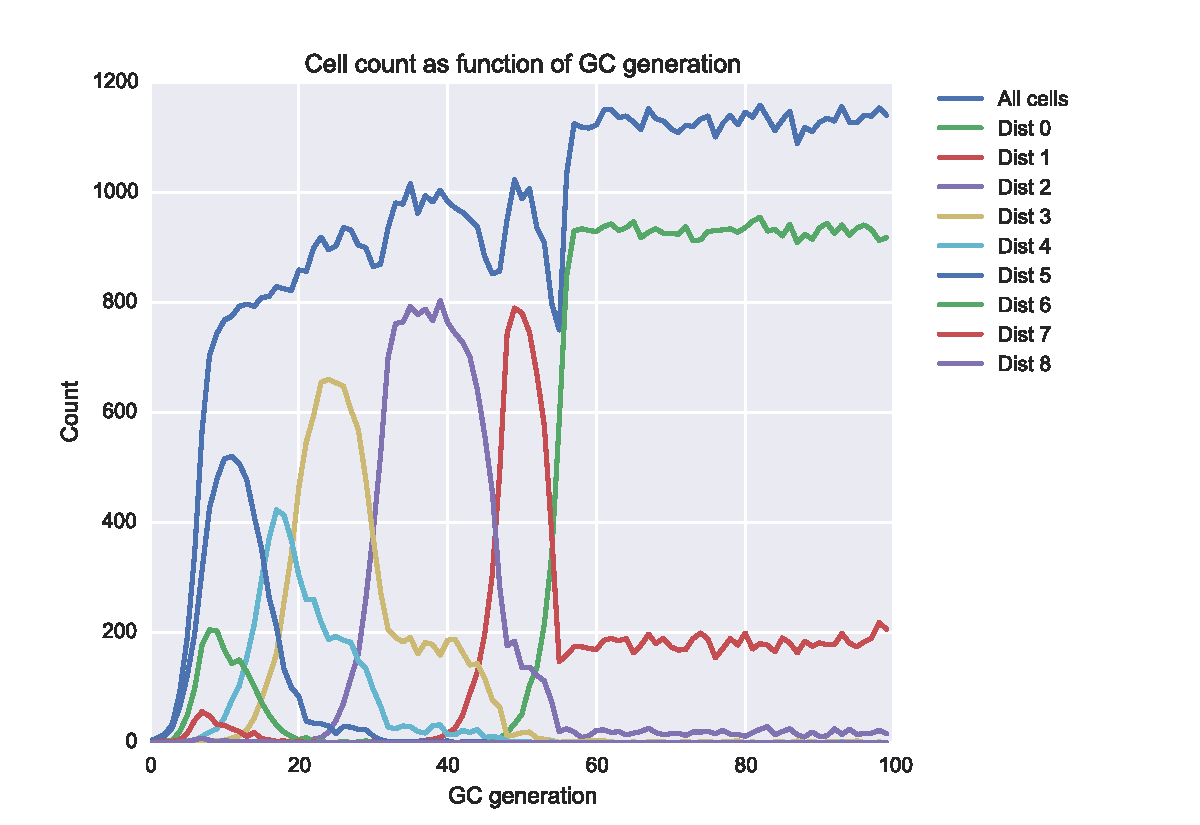
\includegraphics[width=80mm]{figures/sim_selection_default_run_dist5_no_skip.pdf} \newline%
\end{center}
\vspace{-9mm} \hspace{35mm} (a) \hspace{55mm} (b)
    \caption{
        \label{fig:skip_vs_no_skip_dist5}
        Simulation with selection comparing (a) with and (b) without skipping recalculation of $\lambda_i$ at each cell evaluation. In (a) no steps are skipped while, in (b), 99\% of all recalculations are skipped (ten updates to a population of a thousand B cells). In this simulation distance from naive to the mature sequence was 5 and $U$ was set to 2. The rest of the parameters are set to default parameters.
        }
\end{figure}
\fi


Target sequences ($\Tseq_i, i=1,2, \hdots, t_n$) can be arbitrarily defined by inputting a list of amino acid sequences.
Since affinity selection works on the protein level the distance that determines affinity is the Hamming distance between two amino acid sequences.
Either one or multiple target sequences can be used but all are assumed to have equal affinity, $K^{\mature}_d$.
In the tests presented here we input the number of targets ($t_n$) and the amino acid distance from naive seed to target ($t_{\naive}$).
Using these parameters the target sequences are generated by introducing DNA mutations into the naive sequence until it has diverged $t_{\naive}$ away from its starting point.
The mutations are introduced at DNA level by the same neutral branching process described previously, and thereby a distance of $t_{\naive}=10$ does not always correspond to 10 mutations, often the number is higher due to accumulation of synonymous mutations not counting towards protein level distance.
The process is repeated until $t_n$ targets have been made.
We reason that 10 is a good default choice of $t_{\naive}$ achieving sufficient evolutionary distance, however the simulation behaviour seems rather indifferent to this, compare \ref{fig:no_effect_of_f_full} with \ref{fig:skip_vs_no_skip_dist10}.
The default number of targets ($t_n$) is set to 100 to provoke epistatic effects.
All default parameters in the affinity simulation is tabulated in table \ref{aff_constants}.
The implementation is available as a simulation subprogram in the codebase of \texttt{GCtree} (static copy used in this work: \url{github.com/krdav/master_thesis_code}).

\begin{table}[ht]
\centering
\begin{tabular}{lll}
Parameter    & Default & Description \\ \hline
$\lambda_{\mut}$ & None & $\operatorname{Pois}(\lambda_{\mut})$ sequence mutability \\
$T$ & None & Stopping time \\
$cap$ & 1000 & Carrying capacity \\
$t_n$ & 100 & Number of random target sequences \\
$t_{\naive}$ & 10 & Distance from naive to target sequence \\
$n$ & all & Down-sampled number of sequences
\end{tabular}
\caption{
\label{aff_constants}
    Default parameters used in the affinity selected simulations.}
\end{table}










\subsubsection{The epistatic effects of having multiple mature targets}
A BCR is a highly dynamic structure that can bind a single antigen in many different ways, it is therefore also likely that the GC maturation would end up producing different BCRs if replicating the maturation process.
This can be thought of as a multimodal fitness landscape, and it can be emulated by introducing multiple targets into the affinity simulation.
Multimodality in the fitness landscape results in epistasis, which is defined as non additive interaction between mutations, widely observed in nature e.g.\ the evolution of influenza nucleoprotein \cite{gong2013stability}.
The manifestations of epistasis can be different, but here is a simple example where the fitness is shown for various genotypes:
$$
ab = 1,\ Ab = 1,\ aB = 1,\ AB = 10
$$
There are four different genotypes, based on two loci (positions) with two alleles (gene variants), three having a fitness of 1 and one having a fitness of 10.
Each position is tolerable to the two states but only a combination of state $A$ and $B$ improves fitness.
In a linear additive, non epistatic, model setting, the effect of the intermediate states ($Ab$ and $aB$) should sum to the effect of the full state:
$$
ab + (Ab - ab) + (aB -ab) = AB
$$
This is just one example of epistasis, where the effect is AND gate like.
The effect could also confer deleteriousness to an intermediate:
$$
ab = 1,\ Ab = \frac{1}{2},\ aB = \frac{1}{4},\ AB = 10
$$
Or any other non additive influence.

In the affinity simulation there is an inherent epistasis because the transformation from distance to affinity is non-linear, although we could choose to fix $k=1$ in \eqref{eq:hd2affy} to obtain linear additive distance effects.
Regardless, if simulation is done using multiple different targets it will induce epistasis.
The shape of the fitness landscape i.e.\ the distance between modalities, depends on the distance between targets.
Most likely, when two targets are generated they will be $2 \times t_{\naive}$ apart, but sometimes they have overlapping substitutions squeezing modalities together as illustrated in figure \ref{fig:epistasis}.

\begin{figure}[!ht]
\begin{center}
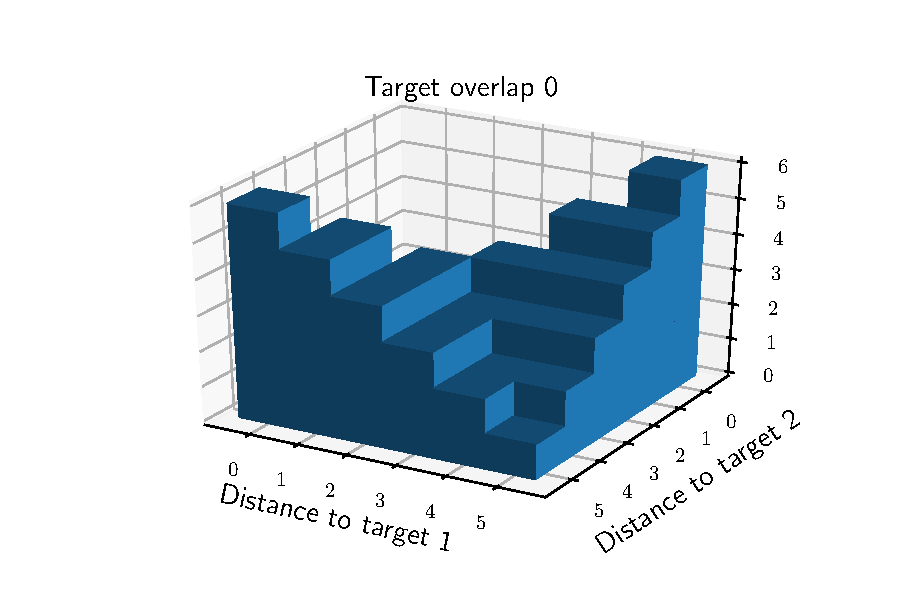
\includegraphics[height=35mm]{figures/fitness_overlap0.pdf}
%\hspace{-40mm}
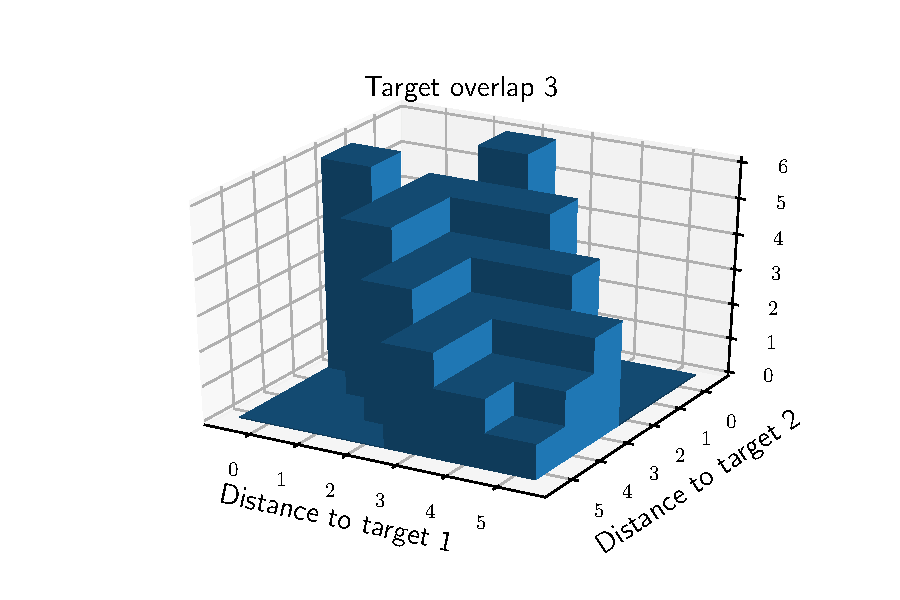
\includegraphics[height=35mm]{figures/fitness_overlap3.pdf}
%\hspace{-40mm}
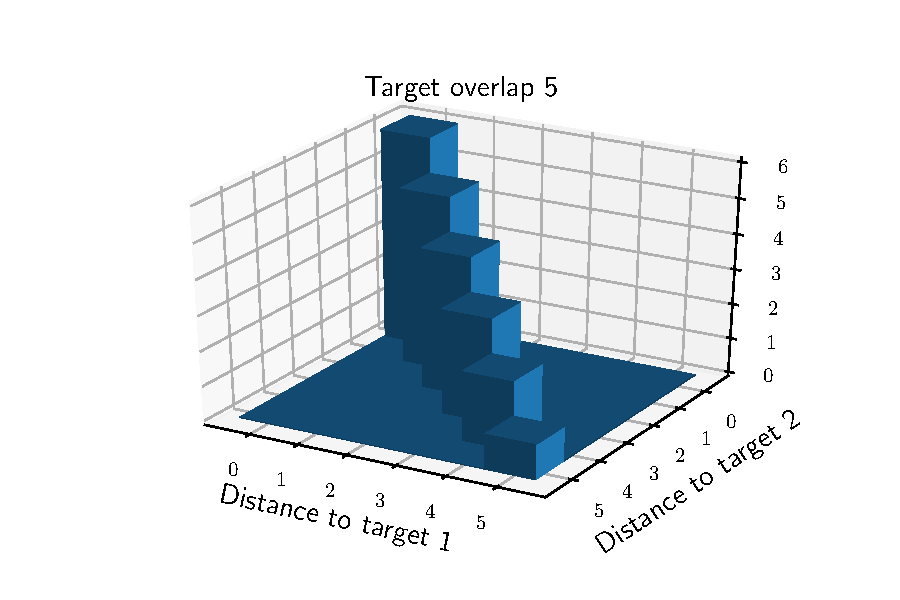
\includegraphics[height=35mm]{figures/fitness_overlap5.pdf} \newline%
\end{center}
\vspace{-6mm} \hspace{26mm} (a) \hspace{39mm} (b) \hspace{39mm} (c)
    \caption{
    \label{fig:epistasis}
        The effect on the fitness landscape of having two target sequences.
        Two target sequences are created with varying overlap using $t_{\naive}=5$.
        The fitness landscape is constructed using a linear distance to affinity function ($k=1$ in \eqref{eq:hd2affy}).
        In a) no overlap makes a long distance between the two fitness peaks, in b) peaks are getting closer when targets overlap, and in c) when the overlap is complete the two targets match and the system no longer is epistatic (assuming a linear distance to affinity function).
        }
\end{figure}


Indeed the effects of epistasis can be observed in simulations with multiple targets.
Often sequences are evolving towards a single target and once a few mutations have been accumulated a sequence is "committed" to this evolutionary trajectory.
However, trajectories can change when a few mutations coincide with another target as observed in figure \ref{fig:epistasis_figure}.
These observations supports the view that the presented affinity simulation is a good challenge to test the assumptions of inference methods.

\begin{figure}[!ht]
    \begin{center}
    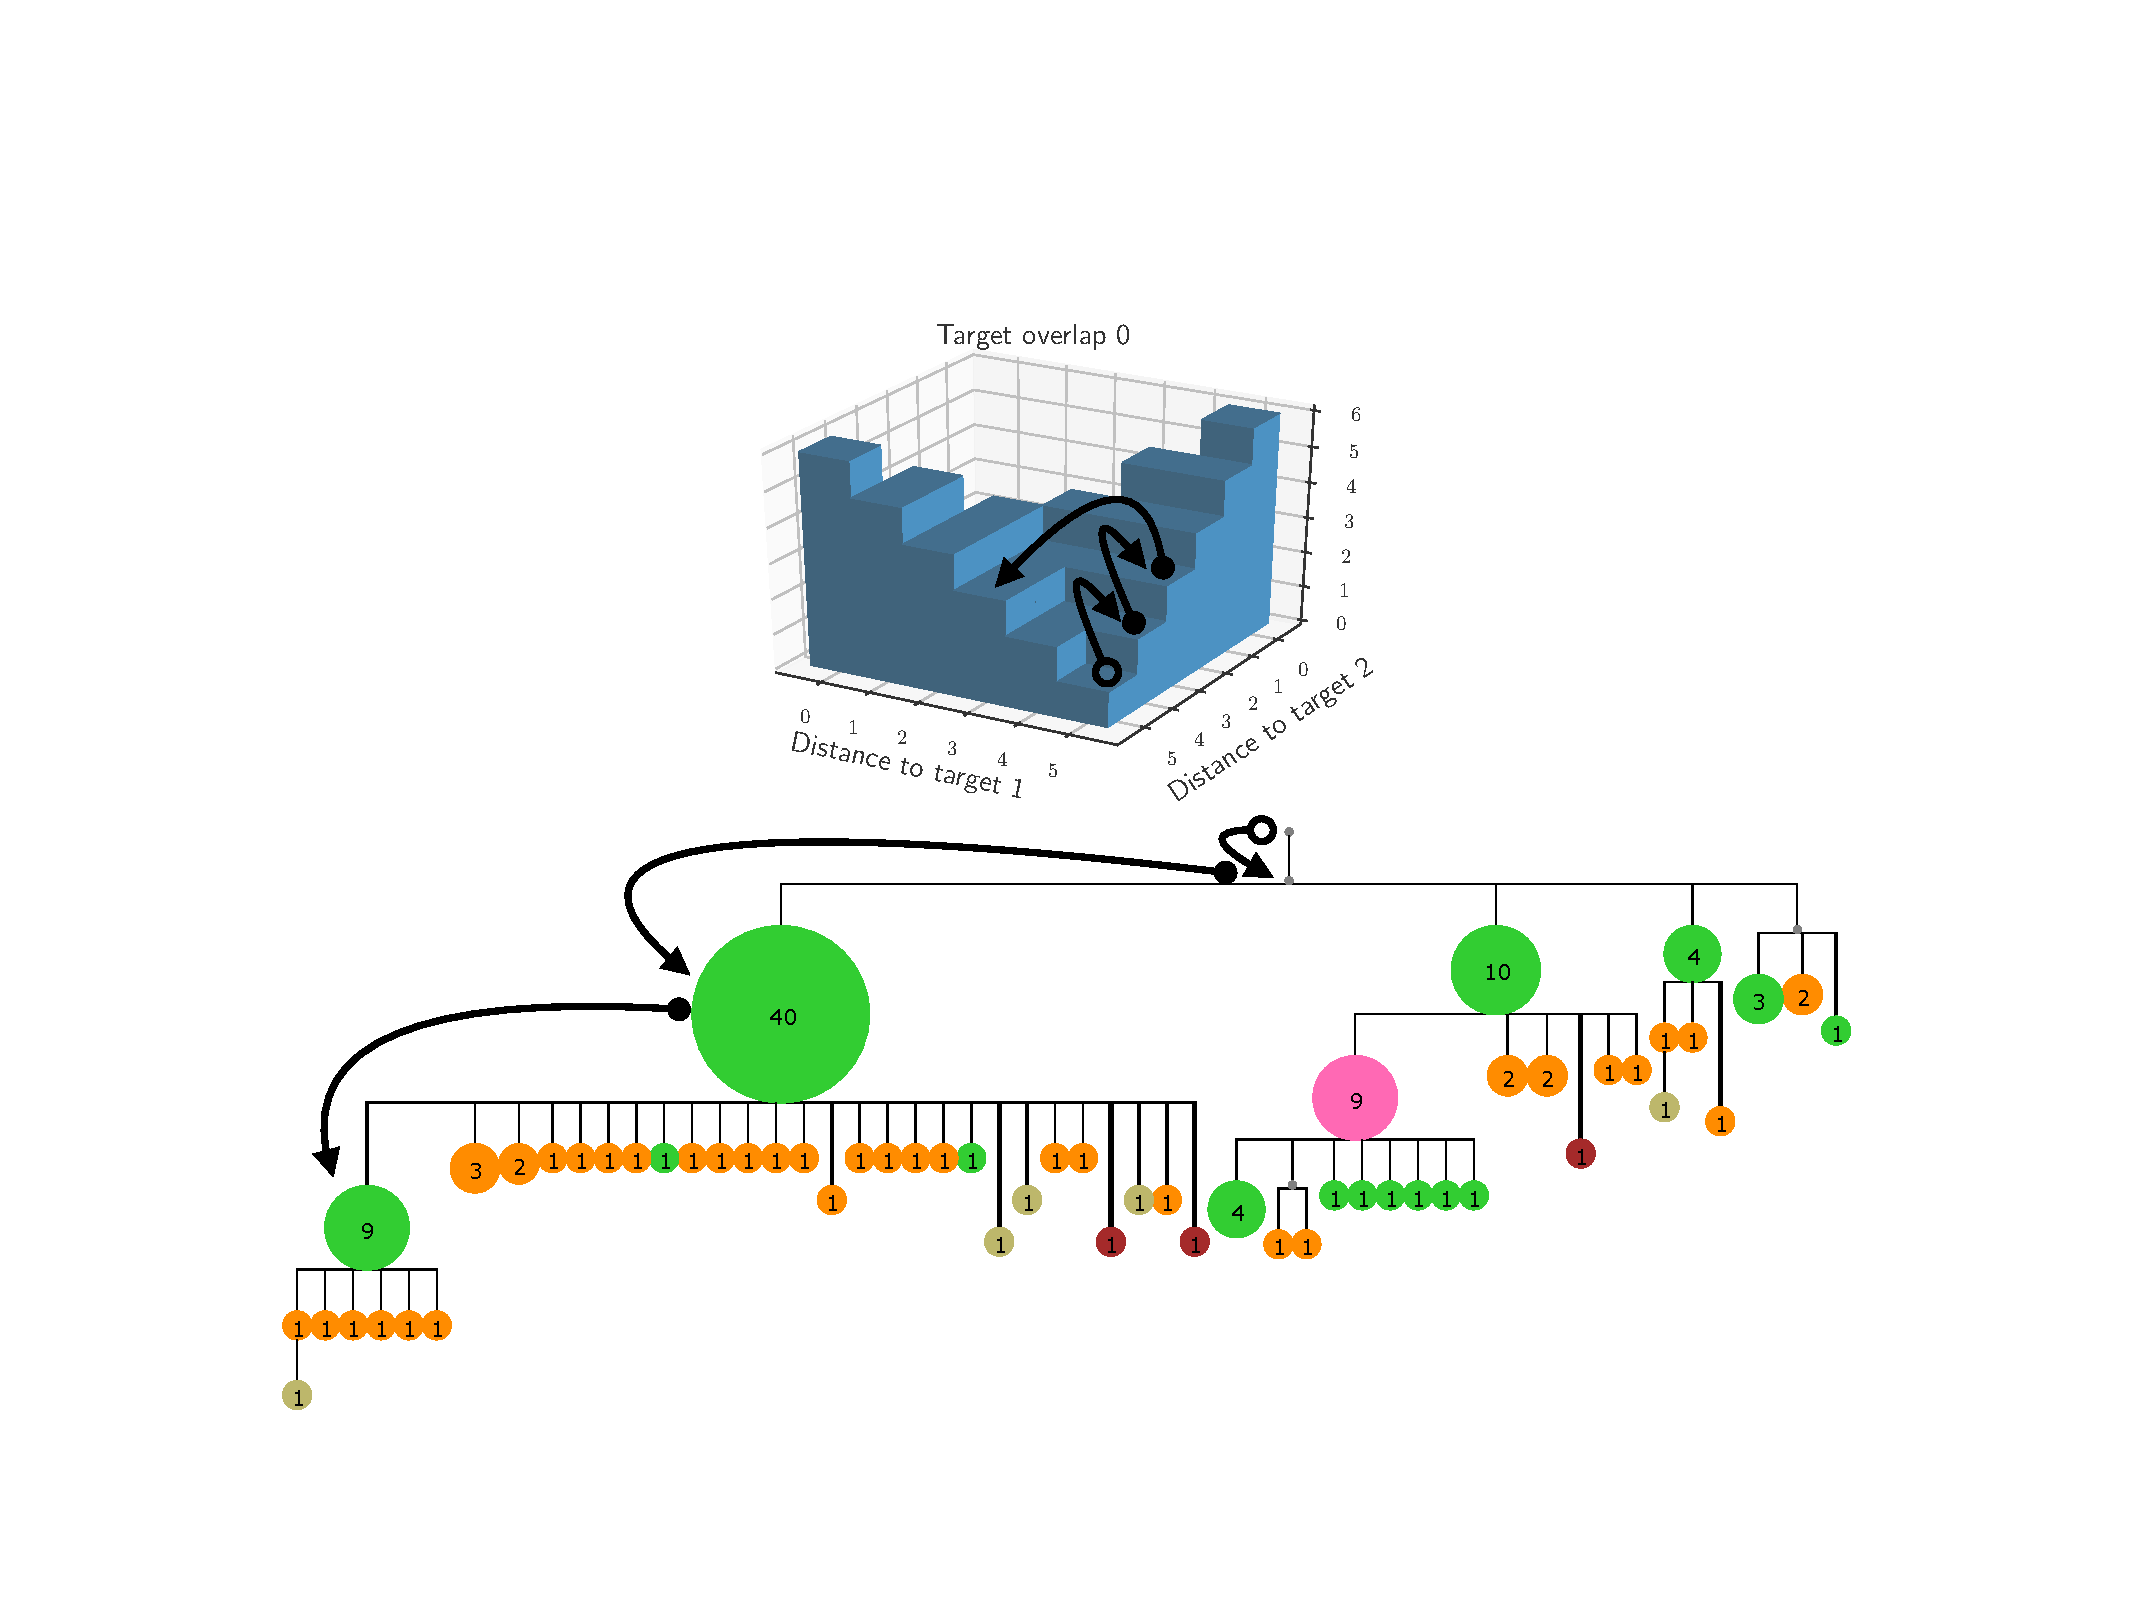
\includegraphics[width=0.8\textwidth]{figures/epistasis_figure.pdf}
        \caption{
        \label{fig:epistasis_figure}
        Example of epistasis in a simulation run with multiple target sequences.
        Colors correspond to the affinity of the simulated cells (figure \ref{fig:collapsed_epistasis} in appendix B for run stats).
        Arrows show an evolutionary trajectory from a low levels in the fitness landscape, starting at the unfilled black circle and progressing to higher levels.
        In the tree, zero amino acid distance branches are collapsed and values inside nodes correspond to the number of B cells.
        We observe a jump between two target sequence trajectories, with the highest frequency node (green 40) yielding a descendant with two amino acid mutations (green 9) that is equally close to another target, resulting in a change in mutational trajectory.
        }
    \end{center}
\end{figure}








%\clearpage
\section{Results}
To test the simulation protocol and whether it recapitulates real world affinity maturation we needed a dataset with a known phylogeny starting from the naive sequence as a root node.
It is practically impossible to get such a dataset, but a an alternative one of the current best single-GC data sets was made by Tas et al.\ \cite{tas2016visualizing}, doing single cells sequencing of B cell isolated from the same GC.
The largest Tas et al.\ clonal family consists of 65 BCR sequences.
Some sequences appear in multiple B cells and these are deduplicated and assigned abundances leaving a total of 42 different genotypes as observed in figure \ref{fig:Tas_tree}.
As a reminder, the phylogeny of the Tas et al.\ dataset is \textit{not} known but inferred based on a likelihood ranking of equally parsimonious trees (unpublished data).

\begin{figure}[!ht]
    \centering
    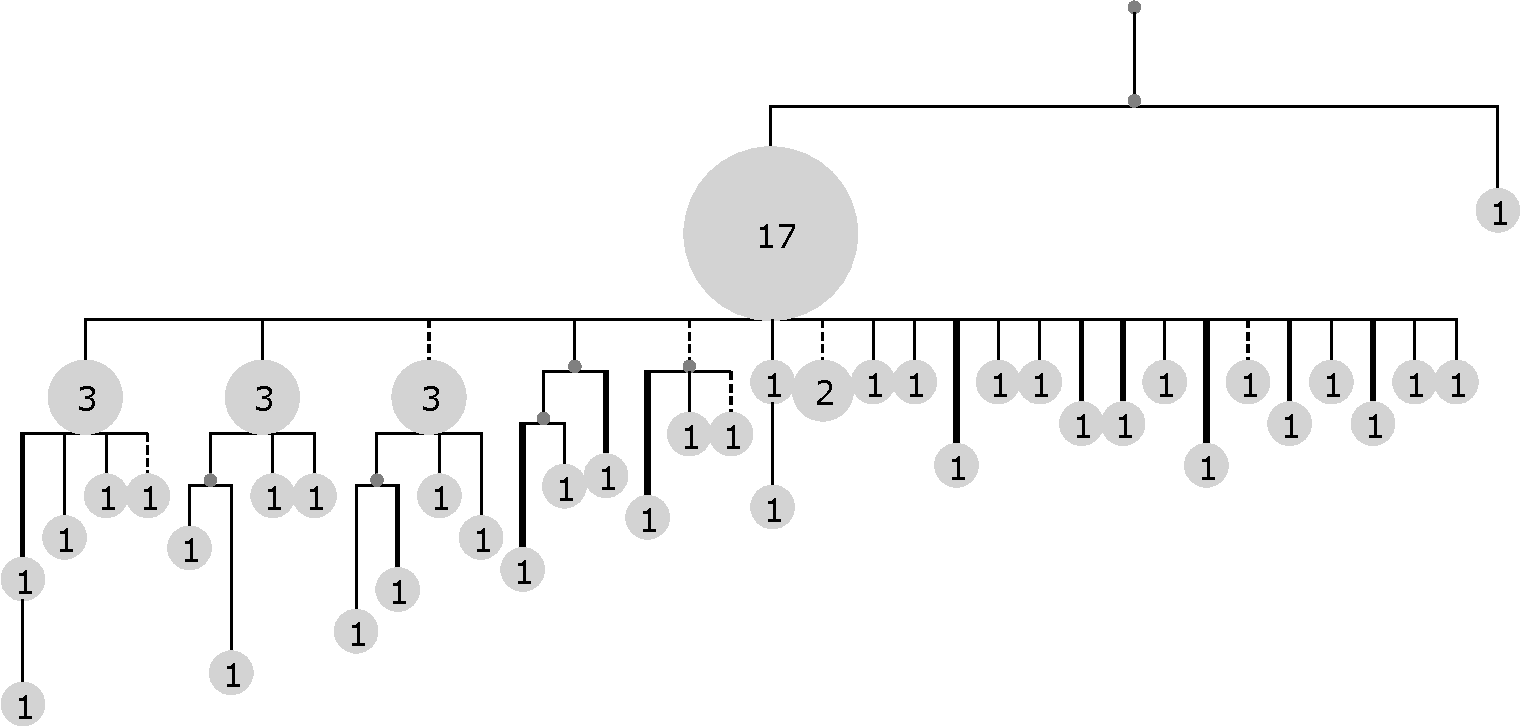
\includegraphics[width=0.8\textwidth]{figures/Tas_tree.pdf}
    \caption{
        \label{fig:Tas_tree}
        Inferred phylogeny for the single GC dataset from Tas et al.\ \cite{tas2016visualizing}.
        The inference method used is based on likelihood ranking of equally parsimonious trees, unpublished but implemented in the \texttt{GCtree} source code as a subprogram.
        Figure credit: William S. DeWitt.
    }
\end{figure}

We would like to tune our simulations to match real data sets as much as possible.
First we need a measure of accumulated SHM, i.e.\ what is the percentage of mutations in the GC sequences, and how is it distributed across the length of the tree.
We plot this mutation distribution as an empirical cumulative distribution function (CDF), see a) in figure \ref{fig:Tas-affsim_Tas-data}.
Next, genotype abundance is an important trait and indicator of clonal bursts.
Higher abundance clones are assumed to be more fit and should therefore also yield more offspring.
Some offspring will have a slightly different genotype and correspondingly different fitnesses, hence high abundance clones should also have many different genotype descendants.
A proxy for counting these descendants is to count the immediate neighbors being just a single Hamming edit away, see b) in figure \ref{fig:Tas-affsim_Tas-data}.
If the assumption holds there should be a positive correlation between abundance and Hamming neighbors.

In figure \ref{fig:Tas-affsim_Tas-data} plotting the two above mentioned measures for the Tas et al.\ dataset, and superimposing the same measures for 100 simulation runs, shows a consistent good fit between simulations and real data.
For this run, parameters were set to $n=65$, $\lambda_{\mut}=0.25$, $t_{\naive}=5$, $T=35$ and default otherwise.
The down-sampling parameter ($n$) was set to the same number as sampled B cells in the Tas et al.\ dataset.
The seed naive sequence used was a V gene of 264 nt; using the commonly cited SHM rate of $10^{-3}$ \cite{victora2012germinal} this gives $\lambda_{\mut}=0.264$ which was rounded to $\lambda_{\mut}=0.25$.
Target distance ($t_{\naive}$) and simulation time ($T$) was adjusted so the simulated sequences had approximately the same minimum Hamming distance to the naive sequence as in the Tas et al.\ dataset (\ref{fig:Tas-affsim_Tas-data}).

\begin{figure}
    \begin{center}
    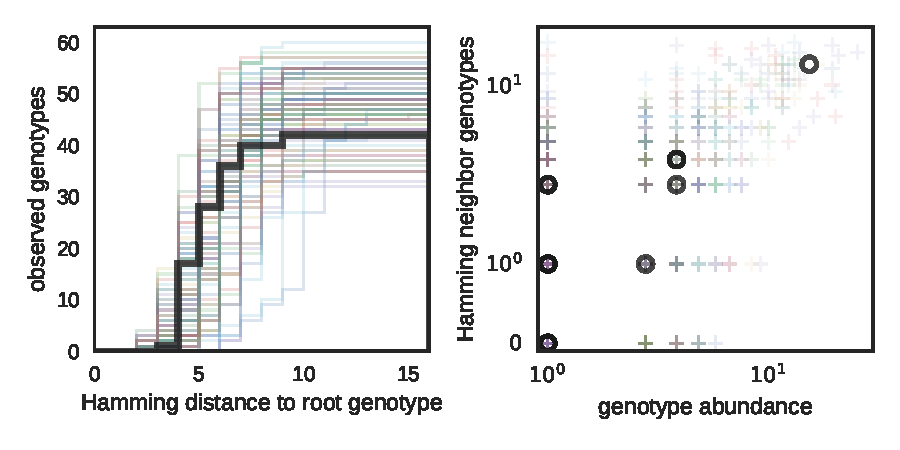
\includegraphics[width=0.8\textwidth]{figures/Tas-affsim_Tas-data.pdf}\newline%
    \end{center}
    \vspace{-14mm} \hspace{42mm} (a) \hspace{52mm} (b)
    \caption{
        \label{fig:Tas-affsim_Tas-data}
        Summary statistics for 100 simulations using $\lambda_{\mut}=0.25$, $t_{\naive}=5$, $T=35$ and $n=65$.
        Simulations are colored and the Tas et al.\ dataset is black.
        In a) the cumulative distribution of mutations (empirical CDF) and b) the number of genotypes in 1 Hamming distance away as function of genotype abundance.
    }
\end{figure}


During affinity simulations the evolution of the cell population was plotted, showing the emergence of new clones with higher affinity and their gradual take over of the cell population, until an even more fit clone emerged (appendix B figure \ref{fig:Tas_affsim_example_with_runstats}).
In all cases of affinity simulation there are a clear progression towards higher affinity as time passes, until eventually a cell has reached the target sequence with highest affinity.
We see that the topology of simulated trees also capture this notion of clonal bursts with one genotype suddenly being very dominant and yielding many offspring (figure \ref{fig:Tas_affsim_example.collapsed_runstat_color_tree}).

\begin{figure}
    \centering
    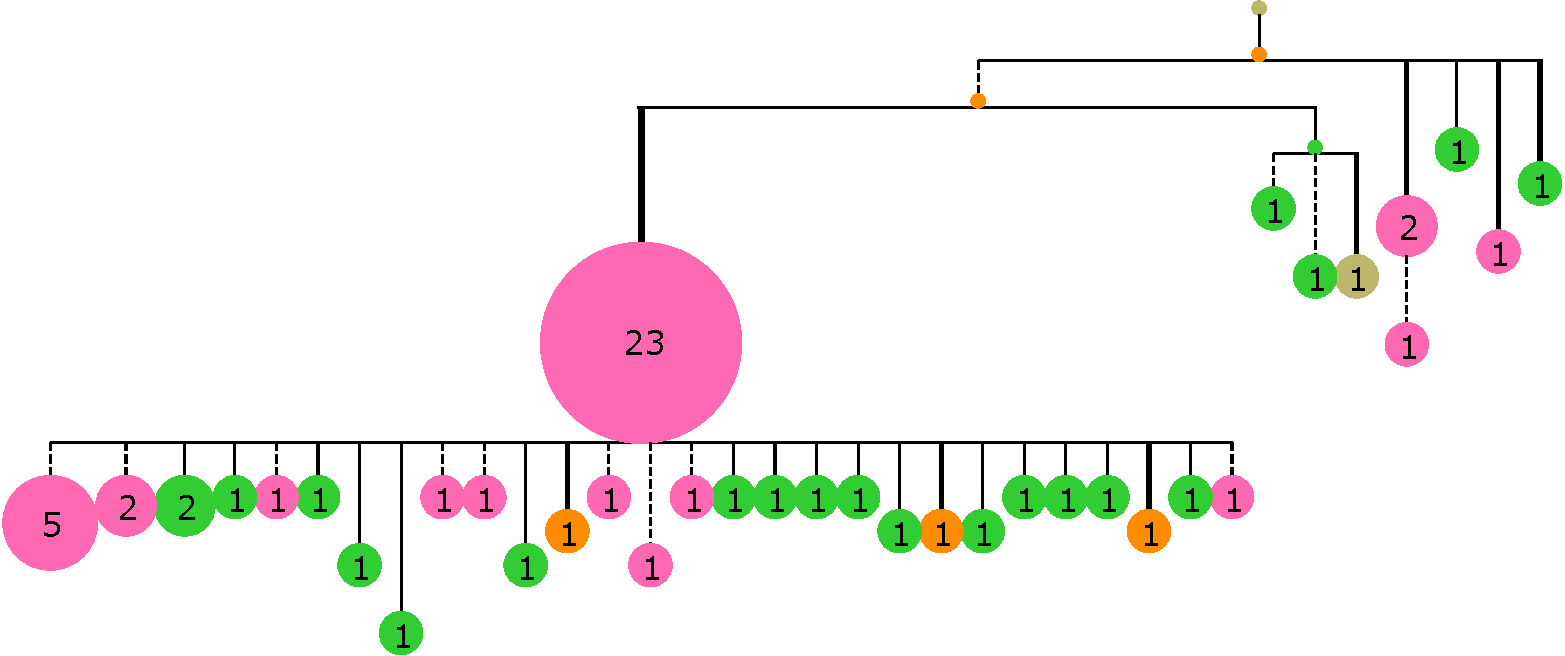
\includegraphics[width=0.8\textwidth]{figures/Tas_affsim_example_collapsed_runstat_color_tree.pdf}
    \caption{
        \label{fig:Tas_affsim_example.collapsed_runstat_color_tree}
        Simulated tree using $\lambda_{\mut}=0.25$, $t_{\naive}=5$, $T=35$ and $n=66$.
        For simulation statistics and color to affinity mapping see appendix B figure \ref{fig:Tas_affsim_example_with_runstats}.
    }
\end{figure}





%%% If doing another iteration of this model I would probably make the fitness a function of antigen bound relative to all the other cells instead of fraction BCRs binding antigen.
% Expressed in equations:
% fitness([AB_i]) = AB_i/sum(AB_i, i from 1 to N)
% In this way it would reflect T cell more realistically, but nevertheless the current model is already capturing most of this relative effect simply by binding more antigen when affinity is increased.
\section{Discussion and conclusion}
Previously, many groups have made models of the GC reaction and affinity maturation \cite{Reshetova_2017}, \cite{Shahaf_2008}, \cite{Chaudhury_2014}, \cite{Wang_Mata_2015}, \cite{Childs_Baskerville_Cobey_2015}, \cite{robert2017simulate}, but none of these have included a definition of the BCR sequences on DNA level.
Neutral branching processes can easily be setup to simulate tree with sequences undergoing the same mutational patterns as real BCRs, but they have no way of capturing the important clonal bursts happening due to the fitness gain from mutating to a higher affinity state.
In the presented work we have addressed this problem through a simple, but yet unexplored way, of integrating affinity based fitness into the simulation of BCR sequence evolution.
We hope that the simulation framework will be a valuable tool in the assessment of inference methods.

It is interesting to see the similarities between the tree topologies of affinity simulated trees, compared to the inferred tree for the Tas et al.\ dataset.
As it was also noted in the work of Tas et al.\ \cite{tas2016visualizing}, this GC has undergone a clonal burst with a single dominant genotype (abundance 17 in figure \ref{fig:Tas_tree}) having many slightly mutated offspring.
Clearly, this topological trait is very similar to a typical affinity simulated tree (figure \ref{fig:Tas_affsim_example_with_runstats}), and in addition by mapping affinities to each node, it can be seen that the clonal burst happened as a result of a mutation conferring higher affinity.
Similarly, Tas et al.\ also observed this characteristic in their experimental data but also noted that the appearance of a high affinity genotype does not guarantee a clonal burst.
This also holds true in the affinity simulation, where under the best conditions a B cell has $\lambda=2$, from which it follows that $\operatorname{Pois}(termination | \lambda=2) = 0.135$, so there is roughly a 14\% chance of a high affinity clone turning extinct.


%The fitness function presented in this model is based on some rough assumptions about having a number of target sequences and using the distance from these as a proxy for affinity.
%However it is possible to plug in an arbitrary fitness function based on empirical values e.g.\ the affinity values determined from ancestral reconstruction of an antibody lineage like Doria-Rose et al.\ \cite{Doria-Rose2014-vi}.


The distribution of clones over time (e.g.\ see appendix B figure \ref{fig:Tas_affsim_example_with_runstats}) reveals that mutations conferring a fitness advantage through affinity increase are quickly found and can quickly overtake the whole GC population.
If this represents the events of real affinity maturation it poses the problem that the probability of completing a maturation trajectory will be defined by the steepness of the fitness function, and not the fitness at the end of a trajectory.
If this is true in nature, it would be a way of leading maturation into a dead end with far lower in fitness than the global optimum, but still too high to be reverted backwards towards the naive sequence.
Indeed such a mechanism is a reasonable, although not the only, explanation why broadly neutralizing HIV antibodies are so rare while their typical germline usage is normal \cite{scheepers2015ability}.

